\documentclass[runningheads]{llncs}

% ---------------------------------------------------------------
% Include basic ECCV package
 
% TODO REVIEW: Insert your submission number below by replacing '*****'
% TODO FINAL: Comment out the following line for the camera-ready version
%\usepackage[review,year=2026,ID=5892]{eccv}
% TODO FINAL: Un-comment the following line for the camera-ready version
%\usepackage[year=2026,ID=5892]{eccv}
\usepackage[preprint]{eccv}

% OPTIONAL: Un-comment the following line for a version which is easier to read
% on small portrait-orientation screens (e.g., mobile phones, or beside other windows)
%\usepackage[mobile]{eccv}


% ---------------------------------------------------------------
% Other packages

% Commonly used abbreviations (\eg, \ie, \etc, \cf, \etal, etc.)
\usepackage{eccvabbrv}

% Include other packages here, before hyperref.
\usepackage{graphicx}
\usepackage{booktabs}

\usepackage{tikz}
\usetikzlibrary{matrix}

% The "axessiblity" package can be found at: https://ctan.org/pkg/axessibility?lang=en
\usepackage[accsupp]{axessibility}  % Improves PDF readability for those with disabilities.


% ---------------------------------------------------------------
% Hyperref package

% It is strongly recommended to use hyperref, especially for the review version.
% Please disable hyperref *only* if you encounter grave issues.
% hyperref with option pagebackref eases the reviewers' job, but should be disabled for the final version.
%
% If you comment hyperref and then uncomment it, you should delete
% main.aux before re-running LaTeX.
% (Or just hit 'q' on the first LaTeX run, let it finish, and you
%  should be clear).

% TODO FINAL: Comment out the following line for the camera-ready version
\usepackage[breaklinks,colorlinks,citecolor=eccvblue]{hyperref}
% TODO FINAL: Un-comment the following line for the camera-ready version
%\usepackage{hyperref}

% Support for ORCID icon
\usepackage{orcidlink}

\usepackage{siunitx}
\DeclareSIUnit{\nothing}{\relax}
\sisetup{
    detect-weight=true, % enable \bfseries to highlight bold values with correct indent
    table-number-alignment = center  % Good alignment with empty cells
}
\usepackage{acronym}
\usepackage{csquotes}
\usepackage{placeins}
\usepackage{makecell}
\usepackage{multirow}
\usepackage{xcolor}
\usepackage{colortbl}
\usepackage{tikz}
\usetikzlibrary{positioning}
\usepackage{xcolor}
\usepackage{colortbl}
\usepackage{array}
\usepackage{makecell}
\usepackage{pifont}
\usepackage{graphicx}
\usepackage{adjustbox}
\usepackage{ifthen}
\usepackage{xparse}
\usetikzlibrary{calc,fit,backgrounds,shapes.arrows,shapes.geometric,decorations.pathreplacing,decorations.text}
\usepackage{tikz-3dplot}
\usepackage{enumitem}
\usepackage{nicefrac}
\usepackage{subcaption}
\usepackage{enumitem}
% Johann prompts
\usepackage[most]{tcolorbox}
\definecolor{darkGreen}{RGB}{22, 119, 53}
\definecolor{lightGreen}{RGB}{198, 226, 208}
\definecolor{myGreen}{RGB}{22, 119, 53}
\usepackage{tabularx}
% Johann Qualitatives
% \usepackage[a4paper,margin=1.5cm]{geometry}
\usepackage{pifont}
\usepackage{tabularx}
\usepackage{array}
\usepackage{booktabs}
\usepackage{pifont}
\usepackage{ragged2e}
\usepackage{subcaption}
\usepackage{adjustbox}
\usepackage{longtable}
% --- inline annotations
%
\newcommand{\go}[1]{\textcolor{gray!70}{#1}}
\newcommand{\red}[1]{{\color{red}#1}}
\newcommand{\todo}[1]{{\color{red}#1}}
\newcommand{\TODO}[1]{\textbf{\color{red}[TODO: #1]}}
\newcommand{\WIP}[1]{\textit{\color{teal}[WIP: #1]}}
\newcommand{\TBD}[1]{\textcolor{red}{\textbf{#1}}}
\newcommand{\missingref}[1]{\textcolor{red}{[REF?]}}
\newcommand{\rb}[1]{\rotatebox{90}{#1}}
\newcommand{\gap}[1]{\makebox[#1]{}}
% --- disable by uncommenting  
% \renewcommand{\TODO}[1]{}
% \renewcommand{\todo}[1]{#1}

\usepackage{pifont}
\newcommand{\cmark}{\ding{51}}
\newcommand{\xmark}{\ding{55}}
\newcommand{\gcmark}{\textcolor{teal}{\ding{51}}}
%\newcommand{\rcmark}{\textcolor{teal}{\ding{51}$^\text{†}$}}
\newcommand{\rcmark}{\textcolor{teal}{(\ding{51})}}
\newcommand{\rxmark}{\textcolor{red}{\ding{55}}}
\newcommand{\gqmark}{\textcolor{gray}{?}}
\newcommand{\up}{\ding{115}}
\newcommand{\aup}{$\uparrow$}
\newcommand{\adown}{$\downarrow$}

\newcommand{\best}[1]{\textbf{#1}}
\newcommand{\second}[1]{\textit{#1}}
%\newcommand{\best}[1]{#1}
%\newcommand{\second}[1]{#1}

\newcommand{\tbf}[1]{\textbf{#1}}
\newcommand{\tul}[1]{\underline{#1}}

\makeatletter
\newcommand\notsotiny{\@setfontsize\notsotiny\@vipt\@viipt}
\makeatother

\newlength{\BenImgWidth}
%\setlength{\BenImgWidth}{43.7mm}
\setlength{\BenImgWidth}{24mm}
\def\arrayStretchFactor{0.97}

% Urban / artificial
\definecolor{UrbanFabric111}{RGB}{230, 0, 77}                     % dark red         #E6004D
\definecolor{UrbanFabric112}{RGB}{255, 102, 102}                  % light red        #FF6666
\definecolor{IndustrialCommercialUnits121}{RGB}{204, 77, 242}     % violet           #CC4DF2
\definecolor{Unlabeled122}{RGB}{204, 204, 204}                    % gray
\definecolor{Unlabeled123}{RGB}{0, 102, 204}                      % blue-gray
\definecolor{Unlabeled124}{RGB}{153, 153, 153}                    % medium gray
\definecolor{Unlabeled131}{RGB}{166, 77, 0}                       % brown
\definecolor{Unlabeled132}{RGB}{102, 51, 0}                       % dark brown
\definecolor{Unlabeled133}{RGB}{255, 153, 51}                     % orange
\definecolor{Unlabeled141}{RGB}{0, 204, 0}                        % bright green
\definecolor{Unlabeled142}{RGB}{102, 255, 102}                    % light green

% Agriculture
\definecolor{ArableLand211}{RGB}{255, 255, 102}                   % yellow           #FFFF66
\definecolor{ArableLand212}{RGB}{204, 255, 102}                   % yellow-green     #CCFF66
\definecolor{ArableLand213}{RGB}{153, 255, 153}                   % pastel green     #99FF99
\definecolor{PermanentCrops221}{RGB}{204, 153, 0}                 % golden brown     #CC9900
\definecolor{PermanentCrops222}{RGB}{255, 204, 102}               % orange-yellow    #FFCC66
\definecolor{PermanentCrops223}{RGB}{153, 204, 0}                 % olive green      #99CC00
\definecolor{Pastures231}{RGB}{204, 255, 153}                     % light lime green #CCFF99
\definecolor{PermanentCrops241}{RGB}{255, 230, 153}               % light beige      #FFE699
\definecolor{ComplexCultivationPatterns242}{RGB}{255, 255, 179}   % pale yellow      #FFFFB3
\definecolor{LandNaturalVegetation243}{RGB}{204, 230, 179}        % pale green       #CCE6B3
\definecolor{AgroForestryAreas244}{RGB}{179, 230, 102}            % muted green      #B3E666

% Forest
\definecolor{BroadLeavedForest311}{RGB}{0, 102, 0}                % dark green       #006600
\definecolor{ConiferousForest312}{RGB}{0, 153, 0}                 % forest green     #009900
\definecolor{MixedForest313}{RGB}{51, 204, 51}                    % medium green     #33CC33

% Shrub / grassland
\definecolor{NaturalGrassland321}{RGB}{204, 255, 204}             % very light green #CCFFCC
\definecolor{MoorsHeathland322}{RGB}{153, 153, 102}               % khaki            #999966
\definecolor{MoorsHeathland323}{RGB}{102, 153, 51}                % olive drab       #669933
\definecolor{TransitionalWoodlandShrub324}{RGB}{153, 204, 153}    % muted green      #99CC99

% Bare areas
\definecolor{BeachesDunesSands331}{RGB}{255, 255, 204}            % sand             #FFFFCC
\definecolor{Unlabeled332}{RGB}{192, 192, 192}                    % light gray       #C0C0C0
\definecolor{NaturalGrassland333}{RGB}{224, 224, 224}             % very light gray  #CCCCCC
\definecolor{Unlabeled334}{RGB}{102, 0, 0}                        % very dark red/brown

% Wetlands
\definecolor{InlandWetlands411}{RGB}{204, 153, 255}               % light purple     #CC99FF
\definecolor{InlandWetlands412}{RGB}{153, 102, 204}               % violet-purple    #9966CC
\definecolor{CoastalWetlands421}{RGB}{204, 204, 255}              % lavender         #CCCCFF
\definecolor{CoastalWetlands422}{RGB}{153, 204, 255}              % light cyan-blue  #99CCFF
\definecolor{Unlabeled423}{RGB}{102, 178, 255}                    % sky blue

% Water
\definecolor{InlandWaters511}{RGB}{0, 128, 255}                   % bright blue     #0080FF
\definecolor{InlandWaters512}{RGB}{0, 0, 204}                     % deep blue       #0000CC
\definecolor{MarineWaters521}{RGB}{51, 153, 255}                  % medium blue     #3399FF
\definecolor{MarineWaters522}{RGB}{0, 204, 255}                   % cyan            #00CCFF
\definecolor{MarineWaters523}{RGB}{0, 51, 153}                    % navy blue       #003399

% Other
\definecolor{Unlabeled999}{RGB}{0, 0, 0}                          % black

\newcommand{\legendbox}[2]{%
  \textcolor{#1}{\rule{1.5ex}{1.5ex}}\,#2%
}
\def\centerarc[#1](#2)(#3:#4:#5)% Syntax: [draw options] (center) (initial angle:final angle:radius)
    { \draw[#1] ($(#2)+({#5*cos(#3)},{#5*sin(#3)})$) arc (#3:#4:#5); }
\newcommand*\circled[1]{\tikz[baseline=(char.base)]{
            \node[shape=circle,draw,inner sep=1pt] (char) {#1};}}

\newcommand{\bentxt}{\texttt{BigEarthNet.txt}}
\newcommand{\bench}{\text{benchmark split}}
%\newcommand{\genExp}{\text{\ac{LULC} expression}}
\newcommand{\genDet}{referring expression detection}
%\newcommand{\pointExp}{point \ac{LULC} expression}
\newcommand{\pointDet}{referring point detection}
%\newcommand{\refExp}{referring \ac{LULC} expression}
\newcommand{\refDet}{referring \ac{LULC} detection}

\newcommand{\clickablelabel}[1]{%
    \stepcounter{enumi}% increment counter
    \llap{\hyperref[#1]{\Alph{enumi}.}}
}

\newcommand{\geochatABBRns}{GC}
\newcommand{\lhrsbotABBRns}{LHRS}
\newcommand{\skyeyegptABBRns}{SE}
\newcommand{\earthdialrgbABBRns}{ED$_\text{rgb}$}
\newcommand{\earthdialmsABBRns}{ED$_\text{s2}$}
\newcommand{\earthmindrgbABBRns}{EM$_\text{rgb}$}
\newcommand{\earthmindmsABBRns}{EM$_\text{s2}$}
\newcommand{\earthmindsarmsABBRns}{EM$_\text{s1s2}$}
\newcommand{\gptABBRns}{GPT}
\newcommand{\qwenABBRns}{Qwen}
\newcommand{\glmABBRns}{GLM}
\newcommand{\llavaABBRns}{LLaVa}
\newcommand{\internvlABBRns}{IVL}
\newcommand{\internvlrsABBRns}{IVL$_{\text{RS}}$}

\newcommand{\geochatABBR}{\geochatABBRns~\cite{kuckreja2024geochat}}
\newcommand{\lhrsbotABBR}{\lhrsbotABBRns~\cite{muhtar2024lhrs}}
\newcommand{\skyeyegptABBR}{\skyeyegptABBRns~\cite{zhan2025skyeyegpt}}
\newcommand{\earthdialrgbABBR}{\earthdialrgbABBRns~\cite{soni2025earthdial}}
\newcommand{\earthdialmsABBR}{\earthdialmsABBRns~\cite{soni2025earthdial}}
\newcommand{\earthmindrgbABBR}{\earthmindrgbABBRns~\cite{shu2025earthmind}}
\newcommand{\earthmindmsABBR}{\earthmindmsABBRns~\cite{shu2025earthmind}}
\newcommand{\earthmindsarmsABBR}{\earthmindsarmsABBRns~\cite{shu2025earthmind}}
\newcommand{\gptABBR}{\gptABBRns~\cite{openai2025gpt5}}
\newcommand{\qwenABBR}{\qwenABBRns~\cite{bai2025qwen3}}
\newcommand{\glmABBR}{\glmABBRns~\cite{hong2025glm}}
\newcommand{\llavaABBR}{\llavaABBRns~\cite{li2024llavaonevision}}
\newcommand{\internvlABBR}{\internvlABBRns~\cite{zhu2025internvl3}}
\newcommand{\internvlrsABBR}{\internvlrsABBRns}

\newcommand{\presenceABBR}{Pr}
\newcommand{\areaABBR}{A}
\newcommand{\countABBR}{Cnt}
\newcommand{\adjacencyABBR}{Adj}
\newcommand{\relativepositionABBR}{RP}
\newcommand{\countryABBR}{Loc}
\newcommand{\seasonABBR}{S}
\newcommand{\climateABBR}{Clt}
\newcommand{\overallABBR}{OA}
\newcommand{\instructionfollowedABBR}{IF}

\renewcommand{\arraystretch}{1.0} % Distance between rows
\setlength{\tabcolsep}{2.3pt} % Distance between columns

% Examples captioning
\definecolor{boxblue}{RGB}{74,138,181}
\definecolor{lightbg}{RGB}{248,248,248}

\newcommand{\ultratiny}{\fontsize{3}{4}\selectfont}
\newcommand{\microfont}{\fontsize{4.2}{5}\selectfont}
\newcommand{\legendfont}{\fontsize{6}{7}\selectfont}
\newcommand{\smallboxfont}{\fontsize{4.4}{5.2}\selectfont}
\newcommand{\bigboxfont}{\fontsize{7}{8.4}\selectfont}
\tikzset{
  captionbox/.style={
    draw=boxblue,
    rounded corners=3pt,
    line width=0.8pt,
    fill=lightbg,
    inner sep=2pt,
    align=left
  },
  row1captionbox/.style={
    captionbox,
    text width=0.28\textwidth
  },
  row2captionbox/.style={
    captionbox,
    text width=0.295\textwidth
  },
  lhrsbox/.style={
    captionbox,
    text width=0.37\textwidth
  },
  % widecaptionbox/.style={
  %   captionbox,
  %   text width=8.5cm
  % },
  hugecaptionbox/.style={
    captionbox,
    text width=12.5cm
  },
  icon/.style={
    circle,
    draw=gray!60,
    fill=white,
    minimum size=7mm,
    inner sep=0pt
  },
  % legendbox/.style={
  %   draw=gray!50,
  %   rounded corners=3pt,
  %   fill=white,
  %   inner sep=4pt
  % }
}

\begin{document}

% ---------------------------------------------------------------
% TODO REVIEW: Replace with your title
\title{BigEarthNet.txt: A Large-Scale Multi-Sensor Image-Text Dataset and Benchmark for Earth Observation} 

% TODO REVIEW: If the paper title is too long for the running head, you can set
% an abbreviated paper title here. If not, comment out.
\titlerunning{BigEarthNet.txt}

% TODO FINAL: Replace with your author list. 
% Include the authors' OCRID for the camera-ready version, if at all possible.
\author{
Johann-Ludwig Herzog\inst{*1}\orcidlink{0009-0001-2294-2301} \and
Mathis Jürgen Adler\inst{*1}\orcidlink{0009-0007-1865-1492} \and
Leonard Hackel\inst{1}\orcidlink{0000-0002-5831-1237} \and
Yan Shu\inst{2} \and
Angelos Zavras\inst{3}\orcidlink{0009-0008-2788-1940} \and
Ioannis Papoutsis\inst{3} \and
Paolo Rota\inst{2} \and
Begüm Demir\inst{1}\orcidlink{0000-0003-2175-7072}
}

% TODO FINAL: Replace with an abbreviated list of authors.
\authorrunning{J.~Herzog et al.}
% First names are abbreviated in the running head.
% If there are more than two authors, 'et al.' is used.

% TODO FINAL: Replace with your institution list.
\institute{BIFOLD and Technische Universität Berlin \and
University of Trento \and
National Technical University and National Observatory of Athens\\
\textsuperscript{*}\notsotiny These authors contributed equally to this work.\\
\vspace{1em}
\normalsize \url{https://txt.bigearth.net}}

\acrodef{AA}{average accuracy}
\acrodef{RGB}{Red-Green-Blue}
\acrodef{AI}{artificial intelligence}
\acrodef{CBIR}{content-based image retrieval}
\acrodef{CL}{contrastive learning}
\acrodef{CLC}{CORINE Land Cover}
\acrodef{CV}{computer vision}
\acrodef{DL}{deep learning}
\acrodef{DEA}{Digital Earth Australia}
\acrodef{EO}{Earth observation}
\acrodef{FLOP}{floating-point operation}
\acrodef{FFN}{feed-forward network}
\acrodef{FM}{foundation model}
\acrodef{mIoU}[mIoU]{mean intersection-over-union}
\acrodef{LLM}{large language model}
\acrodef{LMM}{large multi-modal model}
\acrodef{LULC}{land-use/land-cover}
\acrodef{MAE}{masked autoencoder}
\acrodef{mAP}[mAP$_\mu$]{micro-mean average precision}
\acrodef{MC}{multiple-choice}
\acrodef{MCQ}{multiple-choice question}
\acrodef{MLP}{multi-layer perceptron}
\acrodef{MS}{multispectral}
\acrodef{MTLD}{measure of textual lexical diversity}
\acrodef{NLTK}{Natural Language Toolkit}
\acrodef{NTXent}[NT-Xent]{normalized temperature-scaled cross entropy}
\acrodef{PDF}{probability density function}
\acrodef{RS}{remote sensing}
\acrodef{RTC}{radiometric terrain-corrected}
\acrodef{S1}{Sentinel-1}
\acrodef{S2}{Sentinel-2}
\acrodef{SAR}{synthetic aperture radar}
\acrodef{SOTA}{state-of-the-art}
\acrodef{TCI}{true color image}
\acrodef{ViT}{vision transformer}
\acrodef{VLM}{vision-language model}
\acrodef{VQA}{visual question answering}

\maketitle
% \def\thefootnote{*}\footnotetext{These authors contributed equally to this work}\def\thefootnote{\arabic{footnote}}
\sloppy
\begin{abstract}
\Acp{VLM} have shown strong performance in \ac{CV}, yet their performance on \ac{RS} data remains limited due to the lack of large-scale, multi-sensor \ac{RS} image-text datasets with diverse textual annotations. 
Existing datasets predominantly include aerial \acl{RGB} imagery, with short or weakly grounded captions, and provide limited diversity in annotation types. 
To address this limitation, we introduce \bentxt{}, a large-scale, multi-sensor image-text dataset designed to advance instruction-driven image-text learning in \acl{EO} across multiple tasks. 
\bentxt{} contains \num{464044} co-registered \acl{S1} \acl{SAR} and \acl{S2} \acl{MS} images with \SI{9.6}{\mega\nothing} text annotations, including:
%each associated with: 
i) geographically anchored captions describing \ac{LULC} classes, their spatial relations, and environmental context;
ii) \acl{VQA} pairs relevant for different tasks; and
iii) \genDet{} instructions for bounding box prediction.
Through a comparative statistical analysis, we demonstrate that \bentxt{} surpasses existing \ac{RS} image-text datasets in textual richness and annotation type variety. 
We further establish a manually-verified \bench{} to evaluate \acp{VLM} in \ac{RS} and \ac{CV}. The results show the limitations of these models on tasks that involve complex \ac{LULC} classes, whereas fine-tuning using \bentxt{} results in consistent performance gains across all considered tasks. 
\keywords{ Multi-Sensor Image-Text Dataset \and Vision-Language Models \and Earth Observation \and Remote Sensing }
\end{abstract}   
\acresetall

\section{Introduction}
\label{sec:intro}
    \newcommand{\RingSegment}[6]{%
% #1 = center coordinate
% #2 = inner radius
% #3 = outer radius
% #4 = start angle
% #5 = delta angle
% #6 = TikZ style
\fill[#6]
  (#1) ++(#4:#2)
  arc[start angle=#4, delta angle=#5, radius=#2]
  -- ++(#4+#5:#3-#2)
  arc[start angle=#4+#5, delta angle=-#5, radius=#3]
  -- cycle;
}
\newcommand{\RingLabel}[5]{%
% #1 = center coordinate
% #2 = radius
% #3 = start angle
% #4 = delta angle
% #5 = text
  \pgfmathsetmacro{\angTmp}{#3 + 0.5*#4}
  \pgfmathsetmacro{\rotTmp}{\angTmp}
  \pgfmathsetmacro{\rotTmp}{%
      (\angTmp < 240) ? \angTmp + 180 : ((\angTmp < 300) ? \angTmp + 90 : \angTmp)
    }
  \node[
    font=\bfseries\tiny,
    align=center,
    rotate=\rotTmp
  ] at ($ (#1) + (\angTmp:#2) $) {#5};
}
\newcommand{\RingLabelCurved}[5]{%
% #1 = center
% #2 = radius
% #3 = start angle
% #4 = delta angle
% #5 = text
  \pgfmathsetmacro{\aMid}{#3 + 0.5*#4}
  \path[
    decorate,
    decoration={
      text along path,
      text={|\bfseries\scriptsize|#5},
      text align=center,
      raise=0.5ex
    }
  ]
  (#1) ++(#3:#2)
  arc[start angle=#3, delta angle=#4, radius=#2];
}
\newcommand{\InputOutputBox}[7]{%
    \node[align=justify, anchor=#1, text width=#3, minimum width=#3, minimum height=#2, fill=#4, rounded corners=2mm, font=\fontsize{1pt}{1pt}\selectfont] at (#5) 
          {%
              \textbf{Input:} #6\newline
              \textbf{Output:} #7
    };
}


\begin{figure*}[h!tb]
    \centering

    \begin{tikzpicture}        
        \node[anchor=center] (refMap) at (0,0) {};

        % radii: inner just outside image, outer controls thickness
        \def\rInner{0.4*\BenImgWidth}
        \def\rMid{0.85*\BenImgWidth}
        \def\rOuter{1.25*\BenImgWidth}
        \def\lineSep{1pt}
        \pgfmathsetmacro{\rLabelInner}{1.9}
        \pgfmathsetmacro{\rLabelMid}{2.1}
        \pgfmathsetmacro{\rLabelOuter}{2.5}
        
        \def\aStart{90}
        \def\aBin{136.6}
        \def\aBB{83.1}
        \def\aCap{17.5}
        \def\aMCQ{122.8}
        
        % inner segments
        \RingSegment{refMap}{\rInner}{\rMid}{\aStart}{\aBin}{Orchid!42.5, draw=white, line width=\lineSep}
        \RingSegment{refMap}{\rInner}{\rMid}{\aStart+\aBin}{\aBB}{red!37.5,draw=white,line width=\lineSep}
        \RingSegment{refMap}{\rInner}{\rOuter}{\aStart+\aBin+\aBB}{\aCap}{yellow!50,draw=white,line width=\lineSep}
        \RingSegment{refMap}{\rInner}{\rMid}{\aStart+\aBin+\aBB+\aCap}{\aMCQ}{YellowGreen!40,draw=white,line width=\lineSep}
        \RingLabelCurved{refMap}{\rLabelInner}{\aStart}{\aBin}{Binary VQA}
        \RingLabelCurved{refMap}{0.85*\rLabelInner}{\aStart+\aBin}{\aBB}{Ref. Exp.}
        \RingLabelCurved{refMap}{\rLabelInner}{\aStart+\aBin}{\aBB}{Detection}
        \RingLabel{refMap}{\rLabelMid}{\aStart+\aBin+\aBB}{\aCap}{Captioning}
        \RingLabelCurved{refMap}{\rLabelInner}{\aStart+\aBin+\aBB+\aCap}{\aMCQ}{Multiple-Choice VQA}

        \def\bBinAdj{31.8}
        \def\bBinArea{34.9}
        \def\bBinCount{34.9}
        \def\bBinPresence{34.9}
        \RingSegment{refMap}{\rMid}{\rOuter}{\aStart}{\bBinAdj}{Orchid!15, draw=white, line width=\lineSep}
        \RingSegment{refMap}{\rMid}{\rOuter}{\aStart+\bBinAdj}{\bBinArea}{Orchid!30, draw=white, line width=\lineSep}
        \RingSegment{refMap}{\rMid}{\rOuter}{\aStart+\bBinAdj+\bBinArea}{\bBinCount}{Orchid!45, draw=white, line width=\lineSep}
        \RingSegment{refMap}{\rMid}{\rOuter}{\aStart+\bBinAdj+\bBinArea+\bBinCount}{\bBinPresence}{Orchid!60, draw=white, line width=\lineSep}
        \RingLabel{refMap}{\rLabelOuter}{\aStart}{\bBinAdj}{\adjacencyABBR}
        \RingLabel{refMap}{\rLabelOuter}{\aStart+\bBinAdj}{\bBinArea}{\areaABBR}
        \RingLabel{refMap}{\rLabelOuter}{\aStart+\bBinAdj+\bBinArea}{\bBinCount}{\countABBR}
        \RingLabel{refMap}{\rLabelOuter}{\aStart+\bBinAdj+\bBinArea+\bBinCount}{\bBinPresence}{\presenceABBR}
        
        \def\bBBPoint{43.1}
        \def\bBBRef{40.0}
        \RingSegment{refMap}{\rMid}{\rOuter}{\aStart+\aBin}{\bBBPoint}{red!25,draw=white,line width=\lineSep}
        \RingSegment{refMap}{\rMid}{\rOuter}{\aStart+\aBin+\bBBPoint}{\bBBRef}{red!50,draw=white,line width=\lineSep}
        \RingLabel{refMap}{\rLabelOuter}{\aStart+\aBin}{\bBBPoint}{Ref. Point\\Detection}
        \RingLabel{refMap}{\rLabelOuter}{\aStart+\aBin+\bBBPoint}{\bBBRef}{Ref. LULC\\Detection}
        
        \def\bCap{17.5}
        
        \def\bMCQAdj{14.3}
        \def\bMCQArea{17.5}
        \def\bMCQClimate{17.5}
        \def\bMCQCount{17.5}
        \def\bMCQCountry{17.5}
        \def\bMCQPresence{17.5}
        \def\bMCQRelPos{3.7}
        \def\bMCQSeason{17.5}
        \RingSegment{refMap}{\rMid}{\rOuter}{\aStart+\aBin+\aBB+\aCap}{\bMCQAdj}{YellowGreen!10,draw=white,line width=\lineSep}
        \RingSegment{refMap}{\rMid}{\rOuter}{\aStart+\aBin+\aBB+\aCap+\bMCQAdj}{\bMCQArea}{YellowGreen!20,draw=white,line width=\lineSep}
        \RingSegment{refMap}{\rMid}{\rOuter}{\aStart+\aBin+\aBB+\aCap+\bMCQAdj+\bMCQArea}{\bMCQClimate}{YellowGreen!30,draw=white,line width=\lineSep}
        \RingSegment{refMap}{\rMid}{\rOuter}{\aStart+\aBin+\aBB+\aCap+\bMCQAdj+\bMCQArea+\bMCQClimate}{\bMCQCount}{YellowGreen!40,draw=white,line width=\lineSep}
        \RingSegment{refMap}{\rMid}{\rOuter}{\aStart+\aBin+\aBB+\aCap+\bMCQAdj+\bMCQArea+\bMCQClimate+\bMCQCount}{\bMCQCountry}{YellowGreen!50,draw=white,line width=\lineSep}
        \RingSegment{refMap}{\rMid}{\rOuter}{\aStart+\aBin+\aBB+\aCap+\bMCQAdj+\bMCQArea+\bMCQClimate+\bMCQCount+\bMCQCountry}{\bMCQPresence}{YellowGreen!60,draw=white,line width=\lineSep}
        \RingSegment{refMap}{\rMid}{\rOuter}{\aStart+\aBin+\aBB+\aCap+\bMCQAdj+\bMCQArea+\bMCQClimate+\bMCQCount+\bMCQCountry+\bMCQPresence}{\bMCQRelPos}{YellowGreen!70,draw=white,line width=\lineSep}
        \RingSegment{refMap}{\rMid}{\rOuter}{\aStart+\aBin+\aBB+\aCap+\bMCQAdj+\bMCQArea+\bMCQClimate+\bMCQCount+\bMCQCountry+\bMCQPresence+\bMCQRelPos}{\bMCQSeason}{YellowGreen!80,draw=white,line width=\lineSep}
        \RingLabel{refMap}{\rLabelOuter}{\aStart+\aBin+\aBB+\aCap}{\bMCQAdj}{\adjacencyABBR}
        \RingLabel{refMap}{\rLabelOuter}{\aStart+\aBin+\aBB+\aCap+\bMCQAdj}{\bMCQArea}{\areaABBR}
        \RingLabel{refMap}{\rLabelOuter}{\aStart+\aBin+\aBB+\aCap+\bMCQAdj+\bMCQArea}{\bMCQClimate}{\climateABBR}
        \RingLabel{refMap}{\rLabelOuter}{\aStart+\aBin+\aBB+\aCap+\bMCQAdj+\bMCQArea+\bMCQClimate}{\bMCQCount}{\countABBR}
        \RingLabel{refMap}{\rLabelOuter}{\aStart+\aBin+\aBB+\aCap+\bMCQAdj+\bMCQArea+\bMCQClimate+\bMCQCount}{\bMCQCountry}{\countryABBR}
        \RingLabel{refMap}{\rLabelOuter}{\aStart+\aBin+\aBB+\aCap+\bMCQAdj+\bMCQArea+\bMCQClimate+\bMCQCount+\bMCQCountry}{\bMCQPresence}{\presenceABBR}
        \RingLabel{refMap}{\rLabelOuter}{\aStart+\aBin+\aBB+\aCap+\bMCQAdj+\bMCQArea+\bMCQClimate+\bMCQCount+\bMCQCountry+\bMCQPresence}{\bMCQRelPos}{\relativepositionABBR}
        \RingLabel{refMap}{\rLabelOuter}{\aStart+\aBin+\aBB+\aCap+\bMCQAdj+\bMCQArea+\bMCQClimate+\bMCQCount+\bMCQCountry+\bMCQPresence+\bMCQRelPos}{\bMCQSeason}{\seasonABBR}

        \begin{scope}
          \clip[rounded corners=5mm]
            ($(refMap)+(-0.5*\BenImgWidth,-0.5*\BenImgWidth)$)
            rectangle
            ($(refMap)+( 0.5*\BenImgWidth, 0.5*\BenImgWidth)$);
        
          \node[anchor=center, inner sep=0pt] at (refMap)
            %{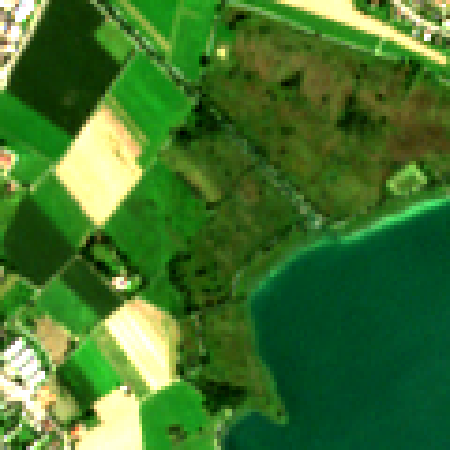
\includegraphics[width=\BenImgWidth]{figures/dataset/samples/_tci_S2A_MSIL2A_20170818T103021_N9999_R108_T32TMT_61_44.png}};
            {\begin{tikzpicture}[scale=0.9]
  % outer disk
  \fill[BlueGreen!20] (0,0) circle (1.2);
  \draw[white, line width=1pt] (0,0) circle (1.2);
  \draw[BlueGreen!50, line width=0.6pt] (0,0) circle (1);

  % latitude / longitude hints
  \draw[BlueGreen!60, line width=0.6pt] (-1.0,0) arc (180:360:1.0 and 0.35);
  \draw[BlueGreen!40, line width=0.3pt, dashed] (-1.0,0) arc (180:0:1.0 and 0.35);
  
  
  \draw[BlueGreen!40, line width=0.3pt, dashed] (0,-1.0) arc (-90:90:0.35 and 1.0);
  \draw[BlueGreen!60, line width=0.6pt] (0,-1.0) arc (-90:-270:0.35 and 1.0);

  
  \draw[BlueGreen!50, line width=0.6pt] (0,0) circle (1);


  % text bars (.txt)
  \node at (-0.6, 0) {
\includegraphics[scale=0.021,decodearray={0 0.65 0 0.65 0 0.65}]{figures/ben_txt_logos/rsim_logo_weiss.png}};
  \fill[gray!70] (-0.2,-0.2) rectangle (0.8,-0.12);
  \fill[gray!70] (-0.2,-0.05) rectangle (0.65,0.03);
  \fill[gray!70] (-0.2,0.10) rectangle (0.75,0.18);

  % name
  %\node[font=\bfseries\scriptsize] at (0,-0.55) {BigEarthNet};
  \path[decorate,decoration={text along path,text={|\bfseries\notsotiny|BigEarthNet},text align=center,raise=-1.6ex}] (-1.0,0) arc (180:360:1.0 and 0.35);
  \node[font=\bfseries\small] at (0,-0.8) {\texttt{.txt}};
\end{tikzpicture}};
        \end{scope}
        
        \def\boxHeight{18mm}
        \def\boxWidth{20mm}  % 20mm
        \InputOutputBox{south east}{0.7*\boxHeight}{\boxWidth}{YellowGreen!60}{$(-\rOuter, -\rOuter) + (-.1,0)$}{Which season is shown in the satellite image? a)~Spring, b)~Summer, c)~Winter, d)~Autumn}{b}
        \InputOutputBox{north east}{0.7*\boxHeight}{\boxWidth}{Orchid!60}{$(-\rOuter, 0) + (-.1,-.05)$}{Are there regions of coastal wetlands in the satellite image?}{No}
        \InputOutputBox{south east}{0.7*\boxHeight}{\boxWidth}{Orchid!15}{$(-\rOuter, 0) + (-.1,.05)$}{Does any inland water border inland wetlands in this scene?}{Yes}
        \InputOutputBox{north east}{0.86*\boxHeight}{\boxWidth}{YellowGreen!40}{$(-\rOuter, \rOuter) + (-.1,0)$}{How many areas covered by urban fabric can be seen? a)~More than five, b)~3, c)~1, d)~0}{b}
        
        \InputOutputBox{south west}{\boxHeight}{\boxWidth}{red!25}{$(\rOuter, -\rOuter) + (.1,-.1)$}{Output a bounding box enclosing the land cover class instance positioned at <point>(0.83, 0.06)</point>.}{[0.49 0.0, 1.0 0.2]}
        \InputOutputBox{west}{\boxHeight}{\boxWidth}{red!50}{$(\rOuter, 0) + (.1,-.05)$}{Where can the <ref>largest area of urban fabric</ref> be found?}{[0.0 0.55, 0.2 1.0]}
        \InputOutputBox{north west}{\boxHeight}{\boxWidth}{YellowGreen!70}{$(\rOuter, \rOuter) + (.1,0)$}{What is the relative position of the arable land to the inland waters? a) to the left, b) to the bottom, c) to the top-right, d) to the top}{a}

        %\InputOutputBox{south}{\BenImgWidth}{64mm+2*\boxWidth-2*25mm}{yellow!50}{$(0, \rOuter) + (0,.1)$}{Describe the content of the image, including the region, climate zone, and land cover distribution.}{This satellite image, captured during the summer season in Switzerland, showcases a diverse landscape within the "temperate, no dry season, warm summer" climate zone. The dominant features are arable land (~526,000 sqm) and inland wetlands (~460,000 sqm), which are adjacent to each other. The arable land borders both inland wetlands and urban fabric (~149,000 sqm). Moreover, the inland wetlands are adjacent to both inland waters (~305,000 sqm) and urban fabric. Notably, the urban fabric is distributed over three individual marginal areas. The varied landscape presents a mix of agricultural areas, wetlands, water bodies, and artificial surfaces.}
        \InputOutputBox{south}{\BenImgWidth}{64mm+2*\boxWidth-2*24mm}{yellow!50}{$(0, \rOuter) + (0,.1)$}{Describe the content of the image, including the region, climate zone, and land cover distribution.}{This satellite image, captured during the summer season in Switzerland, showcases a diverse landscape within the "temperate, no dry season, warm summer" climate zone. The dominant features are arable land ($\sim$526,000 sqm) [...] are adjacent to both inland waters ($\sim$305,000 sqm) and urban fabric. Notably, the urban fabric is distributed over three individual marginal areas. The varied landscape presents a mix of agricultural areas, wetlands, water bodies, and artificial surfaces.}

        \begin{scope}
          % \clip[rounded corners=5mm]
          %   ($(-\rOuter, \rOuter) + (0,.1)$)
          %   rectangle
          %   ($(-\rOuter, \rOuter)+(-\BenImgWidth, \BenImgWidth) + (0,.1)$);
        
          \node[anchor=south east, inner sep=0pt] at ($(-\rOuter, \rOuter) + (0,.1)$)
            {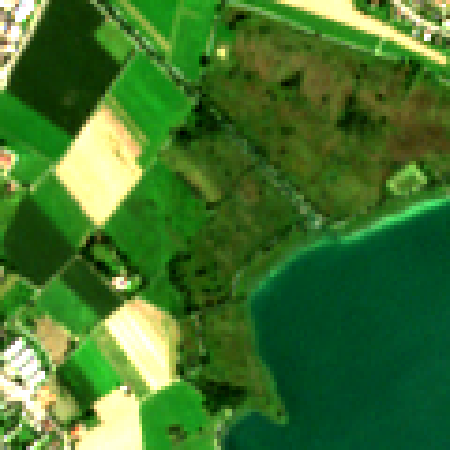
\includegraphics[width=\BenImgWidth]{figures/dataset/samples/_tci_S2A_MSIL2A_20170818T103021_N9999_R108_T32TMT_61_44.png}};
        \end{scope}
        \begin{scope}
          % \clip[rounded corners=5mm]
          %   ($(\rOuter, \rOuter) + (0,.1)$)
          %   rectangle
          %   ($(\rOuter, \rOuter)+(\BenImgWidth, \BenImgWidth) + (0,.1)$);
        
          \node[anchor=south west, inner sep=0pt] at ($(\rOuter, \rOuter) + (0,.1)$)
            {
\includegraphics[width=\BenImgWidth]{figures/dataset/samples/_rtc_S2A_MSIL2A_20170818T103021_N9999_R108_T32TMT_61_44.png}};
        \end{scope}
    \end{tikzpicture} 

    \caption{\bentxt{} comprises \num{464 044} co-registered \ac{S1} and \ac{S2} images with diverse text annotations, resulting in a total of $\sim~\num{9.6}$ million \ac{S1}-\ac{S2}-text triplets. The dataset supports 15 tasks (Presence, Area, Counting, Adjacency, Relative Position, Country, Season, and Climate Zone, denoted as \presenceABBR, \areaABBR, \countABBR, \adjacencyABBR, \relativepositionABBR, \countryABBR, \seasonABBR, and \climateABBR, respectively) across 4 broad categories.}
    \label{fig:dataset_overview}
\end{figure*}
Unprecedented advances in satellite technology have led to a significant increase in the volume of \ac{EO} data archives (\eg the Sentinel satellites of the Copernicus program alone acquire roughly 20~TB of satellite images per day).
In this data-rich landscape, natural language provides an intuitive interface for querying and interpreting these vast \ac{EO} archives, with \acp{VLM} emerging as an effective framework for jointly encoding visual observations and natural language for tasks such as image captioning~\cite{cheng2022nwpu, hoxha2020toward, sumbul2020sd}, \ac{VQA}~\cite{lobry2020rsvqa, chappuis2022prompt, hackel2023lit} and \genDet~\cite{kuckreja2024geochat, soni2025earthdial, zhan2025skyeyegpt}.

In general, \acp{VLM} are applied to \ac{EO} data either by using general-purpose \ac{CV} \acp{VLM} directly or by training \ac{RS}-specific \acp{VLM}.
The first approach is limited by the fundamentally different spectral and spatial characteristics between the \ac{CV} and \ac{RS} images. For example, the \ac{S2} \ac{MS} images comprise 13 spectral bands associated with varying spatial resolutions, while those in \ac{CV} include \ac{RGB} bands in general. The high spectral resolution data enable the discrimination of complex \ac{LULC} classes in RS. Although \ac{RGB} information may be sufficient to distinguish generic classes, \eg,\enquote{Water} from \enquote{Forests and seminatural areas}, additional spectral information beyond the visible spectrum is needed to differentiate complex \ac{LULC} classes, \eg, \enquote{Mixed forest} vs. \enquote{Coniferous forest}~\cite{sumbul2019bigearthnet}. Due to their pretraining phase using \ac{RGB}-only image-text data, the \acp{VLM} in \ac{CV} have limited capability to effectively query and interpret RS data. Although several \ac{RS}-specific \acp{VLM} trained on \ac{RS} image-text datasets~\cite{bazi2024rsllava, zhan2025skyeyegpt, kuckreja2024geochat, muhtar2024lhrs} have recently been developed, most of these models are still trained only on \ac{RGB} data and thus subject to the above-mentioned limitations. It is worth noting that there are only a few works that include multispectral or multi-sensor (e.g., multispectral, \ac{SAR})  image-text data during pre-training~\cite{shu2025earthmind, soni2025earthdial}. The use of multi-sensor data is particularly crucial, since different satellite sensors have the capability of measuring different physical properties of \ac{LULC} classes and their joint use can improve task performance ~\cite{sumbul2021bigearthnet, hong2020more, Sumbul_2025_ICCV}.
However, as shown in \cref{tab:existing_datasets_properties}, the existing \ac{RS} image-text datasets suffer from: i) limited availability of co-registered multi-sensor data that includes more than three bands, and ii) limited diversity in text annotation types.
These limitations directly hinder the ability of \acp{VLM} to characterize: 1) the complex spatial/spectral content of \ac{RS} images; and also 2) complementary information among multi-sensor data. 
 \begin{table*}[h!tb]
    \centering
    %\small
    \renewcommand{\arraystretch}{\arrayStretchFactor}
    \setlength\tabcolsep{1pt}
    \caption{
    Comparison of existing \ac{RS} image-text datasets. Datasets are compared in terms of: 1) the presence of co-registered multi-sensor imagery exceeding three spectral bands; 2) methods used for text annotation, including the presence of an extensive manual quality check (QC); 3) supported tasks; 4) availability of geolocation data and 5) the number of image-text (IT) samples. 
    \rcmark{} indicates that only parts of the dataset fulfill this property.
    }
    \begin{tabular}{l >{\centering\arraybackslash}p{0.5cm} >{\centering\arraybackslash}p{0.8cm} >{\centering\arraybackslash}p{0.5cm} c >{\centering\arraybackslash}p{0.5cm} >{\centering\arraybackslash}p{0.5cm} >{\centering\arraybackslash}p{0.5cm} >{\centering\arraybackslash}p{0.5cm} >{\centering\arraybackslash}p{0.5cm} c >{\centering\arraybackslash}p{0.5cm} >{\centering\arraybackslash}p{0.5cm} >{\centering\arraybackslash}p{0.8cm} c r}
    \toprule
     \multirow{2}{*}{\makecell{\\[14pt]Dataset}}     & \multicolumn{3}{c}{\makecell{Multi-Sensor\\[-4pt]Images}} && \multicolumn{5}{c}{Annotation Method} && \multicolumn{3}{c}{\makecell{Supported\\[-4pt]Tasks}} & \multirow{2}{*}{\rb{Geolocation data\gap{8pt}}} & \multirow{2}{*}{\rb{\#IT samples\gap{7pt}}}\\
     \cmidrule{2-4} \cmidrule{6-10} \cmidrule{12-14}
                                                     & \multicolumn{1}{c}{\rb{Available}} & \multicolumn{1}{c}{\rb{\makecell{>3 bands\\[-4pt]per image}}} & \multicolumn{1}{c}{\rb{Co-registered}} && \multicolumn{1}{c}{\rb{Manual}} & \multicolumn{1}{c}{\rb{Template}} & \multicolumn{1}{c}{\rb{Web scraped}} & \multicolumn{1}{c}{\rb{LLM-based}} & \multicolumn{1}{c}{\rb{Manual QC}} && \multicolumn{1}{c}{\rb{Captioning}} & \multicolumn{1}{c}{\rb{VQA}} & \multicolumn{1}{c}{\rb{\makecell{Ref. Exp.\\[-4pt]Detection}}}\\
\midrule
                                                     % ms-avail  all-bands ms-paired   manual   template  web       llm       manual-qc  captioning vqa      det       loc      samples
     UCM-Captions~\cite{qu2016deep}                  & \rxmark & \rxmark & \rxmark && \gcmark & \rxmark & \rxmark & \rxmark & \gcmark && \gcmark & \rxmark & \rxmark & \rxmark & 10.5k \\
     Sydney-Captions~\cite{qu2016deep}               & \rxmark & \rxmark & \rxmark && \gcmark & \rxmark & \rxmark & \rxmark & \gcmark && \gcmark & \rxmark & \rxmark & \rxmark & 3k \\
     RSICD~\cite{lu2017exploring}                    & \rxmark & \rxmark & \rxmark && \gcmark & \rxmark & \rxmark & \rxmark & \gcmark && \gcmark & \rxmark & \rxmark & \rxmark & 54.6k \\
     RSITMD~\cite{yuan2022exploring}                 & \rxmark & \rxmark & \rxmark && \gcmark & \rxmark & \rxmark & \rxmark & \gcmark && \gcmark & \rxmark & \rxmark & \rxmark & 23.7k \\
     NWPU-Captions~\cite{cheng2022nwpu}              & \gcmark & \rxmark & \rxmark && \gcmark & \rxmark & \rxmark & \rxmark & \gcmark && \gcmark & \rxmark & \rxmark & \rxmark & 157k \\
     GAIA~\cite{gaia_zavras}                         & \gcmark & \rxmark & \rxmark && \rxmark & \rxmark & \gcmark & \gcmark & \rxmark && \gcmark & \rxmark & \rxmark & \rcmark & 205k \\
     Git-10M~\cite{Text2Earth_git_10m}               & \gcmark & \rxmark & \rxmark && \rxmark & \rxmark & \rxmark & \gcmark & \rxmark && \gcmark & \rxmark & \rxmark & \gcmark & 10.5M \\
     RSVQAxBEN~\cite{lobryRSVQAMeetsBigearthnet2021} & \rxmark & \rxmark & \rxmark && \rxmark & \gcmark & \rxmark & \rxmark & \rxmark && \rxmark & \gcmark & \rxmark & \rxmark & 14.8M \\
     RS5M~\cite{zhang2024rs5m}                       & \gcmark & \rxmark & \rxmark && \rxmark & \rxmark & \rcmark & \rcmark & \rxmark && \gcmark & \rxmark & \rxmark & \rcmark & 5.0M \\
     RSTeller~\cite{ge2025rsteller}                  & \rxmark & \rxmark & \rxmark && \rxmark & \rxmark & \rxmark & \gcmark & \rxmark && \gcmark & \rxmark & \rxmark & \rxmark & 2.6M \\
     Landsat30-AU~\cite{ma2025landsat30}             & \rxmark & \rxmark & \rxmark && \rxmark & \rxmark & \rxmark & \gcmark & \rcmark && \gcmark & \gcmark & \rxmark & \rcmark & 216k \\
     ChatEarthNet~\cite{ChatEarthNet}                & \rxmark & \gcmark & \rxmark && \rxmark & \rxmark & \rxmark & \gcmark & \rcmark && \gcmark & \rxmark & \rxmark & \rxmark & 173k \\
     MS-Clip~\cite{marimo2025beyond}                 & \gcmark & \gcmark & \gcmark && \rxmark & \rxmark & \rxmark & \gcmark & \rxmark && \gcmark & \rxmark & \rxmark & \rxmark & 985k \\
     \bentxt (ours)                                  & \gcmark & \gcmark & \gcmark && \rxmark & \gcmark & \rxmark & \gcmark & \rcmark && \gcmark & \gcmark & \gcmark & \gcmark & 9.6M \\
    \bottomrule
    \end{tabular}
    \label{tab:existing_datasets_properties}
\end{table*}

To overcome the above-mentioned limitations, in this paper we present \bentxt: a large-scale image-text dataset made up of \num{464044} co-registered \acl{S1} \acl{SAR} and \acl{S2} \acl{MS} images with \SI{9.6}{\mega\nothing} text annotations, including captions, \acp{VQA} with varying answer formats, and \genDet{} annotations (see \cref{fig:dataset_overview}). In addition, we introduce a \bench{} that contains \num{1082} image pairs with manually verified text annotations for systematic evaluation of VLMs for EO tasks. Using our \bench{}, we demonstrate that current \acp{VLM} in both \ac{CV} and \ac{RS} show limited ability to characterize the complex content of multi-sensor \ac{RS} images. Fine-tuning a \ac{SOTA} \ac{VLM} (InternVL3-1B~\cite{zhu2025internvl3}) adapted for multi-sensor input (denoted as RS-InternVL) on \bentxt{} leads to substantial performance gains across all considered tasks.

In summary, our contributions are as follows:
\begin{enumerate}
    \item We show that the existing \acp{VLM} from both \ac{CV} and \ac{RS} domains exhibit limited capability to characterize the complex spatial/spectral content of multi-sensor images in \ac{RS}. To this end, we conduct extensive experiments across 15 tasks of 4 categories: image captioning, binary \ac{VQA}, \ac{MCQ}, and \genDet.
    \item We introduce \bentxt{} (which is the first dataset unifying co-registered multi-sensor \ac{RS} data with diverse textual descriptions) together with a manually checked subset (\bench{}).
    \item We adapt InternVL to accommodate multi-sensor RS inputs and perform domain-specific fine-tuning using \bentxt. Our results serve as experimental validation of the critical role of large-scale, multi-sensor image-text datasets for accurate interactions with EO data.
\end{enumerate}

\section{Related work}
\label{sec:related_works}
\Acp{VLM} in \ac{RS} enable natural language interactions with images across multiple tasks, including \ac{VQA}, change captioning, and \genDet{} \cite{kuckreja2024geochat, irvin2025teochat, soni2025earthdial}. To facilitate the research and development of \acp{VLM}, several image-text datasets have been proposed in RS.
Early \ac{RS} image–text datasets, such as UCM-Captions, Sydney-Captions \cite{qu2016deep}, RSICD \cite{lu2017exploring}, RSITMD \cite{yuan2022exploring}, and NWPU-Captions \cite{cheng2022nwpu} contain high-resolution aerial imagery with human-written single-sentence descriptions with limited intra-class diversity. 
To overcome this bottleneck, recently proposed datasets shift toward large-scale, automatically generated texts: RS5M \cite{zhang2024rs5m} introduces the first million-scale corpus with 5 million image–caption pairs; GAIA \cite{gaia_zavras} provides \num{205150} pairs, with multi-sentence captions emphasizing environmental dynamics; and Landsat30-AU \cite{ma2025landsat30} contains \num{196262} image-caption pairs and \num{17725} \ac{MC} \acp{VQA}.
For \ac{VQA} specifically, RSVQA \cite{lobry2020rsvqa} comprises \num{77232} and \num{1066316} question-answer triplets for low- and high-resolution imagery, while RSVQAxBEN \cite{lobryRSVQAMeetsBigearthnet2021} scales to approximately \num{15} million pairs with \ac{S2} BigEarthNet~\cite{sumbul2019bigearthnet} \ac{RGB} composites for \ac{CLC} class presence.
Recent studies also extend the spectral range of image-text datasets beyond \ac{RGB}. 
Yuan et. al~\cite{ChatEarthNet} generate captions for nine-band \ac{S2} images, yet descriptions rely on broad \ac{LULC} classes from ESA WorldCover~\cite{zanaga2022esaworldcover} (\eg water, tree, snow). Marimo et al.~\cite{marimo2025beyond} scale to \num{975000} co-registered \ac{S1}–\ac{S2} images from SSL4EO~\cite{wang2023ssl4eo} but generate captions using a \ac{VLM} that receives \ac{RGB} bands only, preventing texts from relying on information beyond the visible spectrum. 

\section{BigEarthNet.txt Dataset}
\label{sec:bigearth_txt}
To address the scarcity of large-scale multi-sensor image-text datasets in \ac{RS}, we introduce \bentxt{}, which comprises co-registered \ac{S1} and \ac{S2} images with semantically rich natural-language annotations relevant for 15 tasks across 4 broad categories: i)~captioning; ii)~binary and iii)~multiple-choice \ac{VQA}; and iv)~\genDet. The co-registered \ac{S1} and \ac{S2} images in \bentxt{} are taken from BigEarthNet~v2.0~\cite{clasen2025reben}, which comprises \num{549488} pairs of \ac{S1} and \ac{S2} images acquired over ten European countries. Each pair is accompanied by a pixel-level \ac{LULC} reference map based on the \ac{CLC} 2018 product  (\texttt{V2020\_20u1})~\cite{clcbook}. Some images in BigEarthNet~v2.0 are partly covered by seasonal snow, clouds, and cloud shadows, and also associated with reference maps containing unclassified pixels (with no LULC label). To construct our dataset, we filter out such image pairs, resulting in \num{464044} co-registered \ac{S1} and \ac{S2} images. In the following, we describe in detail our annotation generation pipeline, present the caption statistics and then finally introduce our \bench{}.  

\subsection{Annotation Generation Pipeline}
The textual annotations for \bentxt{} are generated through a three-stage pipeline (template-based caption generation, \ac{LLM}-based linguistic augmentation, \ac{VQA} and \ac{LULC} annotation generation). 
An overview of the caption generation and linguistic augmentation stage is given in \cref{fig:caption_generation_process}.
\paragraph{Template-based caption generation.} We first construct captions by extracting four categories of spatial attributes directly from the reference maps: the \textit{presence} of \ac{LULC} classes, the \textit{count} of individual contiguous regions per class (instances), the \textit{size} of each class in total and per instance, and pairwise spatial \textit{adjacency} between classes. 
Area values are rounded to the nearest \SI{1000}{\meter\squared} to reduce label noise. 
Classes are assigned to one of three tiers based on their image coverage:
i)~\textit{primary} (> \SI{25}{\percent}); 
ii)~\textit{secondary} (\SI{5}{\percent} - \SI{25}{\percent}); or
iii)~\textit{marginal} (<\SI{5}{\percent}).
Captions are composed from pre-defined templates that contain classes, sizes, and adjacency relations accordingly. 
Each caption is further grounded in spatio-seasonal context by appending the acquisition season, country, and Köppen-Geiger climate zone~\cite{beckHighresolution1Km2023}, derived from high-resolution climate maps.

\paragraph{LLM-based linguistic augmentation.} Although template-based captions guarantee factual correctness, they exhibit limited linguistic variety. 
Therefore, we apply a two-stage augmentation using the quantized Llama-4-Scout-17B model~\cite{touvron2023llamaopenefficientfoundation}.
First, a \textit{paraphrasing} step diversifies lexical and syntactic structure while prohibiting the addition of unsupported information.
Second, a \textit{self-refinement} step \cite{self-refinement} revises the paraphrased output against the original template to eliminate hallucinated content and restore missing information. 
To further increase valid lexical variation, the prompt includes the \ac{CLC} nomenclature, permitting semantically valid substitutions (\eg referring to \emph{Urban fabric} collectively as \emph{Artificial surfaces}). 
Manual evaluation of \num{3209} randomly sampled augmented captions against four binary criteria (linguistic correctness, factual accuracy, completeness, and absence of generation artifacts) yields an average correctness of \SI{93.76}{\percent}, with \SI{77.50}{\percent} of captions satisfying all four criteria simultaneously.
\begin{figure*}[!ht]
    \centering

    \begin{tikzpicture}        
        \node[inner sep=0pt,minimum size=0pt] (CaptionAnchor) at (-4.7, 0) {};
        \node[single arrow,
              minimum height=40mm, minimum width=20mm,
              single arrow head extend=2mm,
              anchor=west, rotate=-90, fill=gray!15] at (1.33,-4) {};
        \node[anchor=west] (refMap) at (0,0)
            {
\includegraphics[width=\BenImgWidth]{figures/dataset/samples/_ref_map_S2A_MSIL2A_20170818T103021_N9999_R108_T32TMT_61_44.png}};
        \node[anchor=south] (refMapCap) at ($(refMap.north) + (0,-.2)$) {\small\textcolor{gray}{Reference map}};

        \node[align=justify, anchor=south east, text width=30mm, minimum width=30mm, minimum height=20mm, fill=cyan!20, rounded corners=2mm, font=\scriptsize] (PresenceSizeTemplate) at ($(refMap.north west) + (-.2,.2)$) {This image primarily shows \textbf{[class]} (\textbf{[size]})... Smaller areas are occupied by \textbf{[class]} (\textbf{[size]}) and \textbf{[class]} (\textbf{[size]}).};
        
        \node[align=justify, anchor=south west, text width=30mm, minimum width=30mm, minimum height=20mm, fill=WildStrawberry!20, rounded corners=2mm, font=\scriptsize] (SizeCountTemplate) at ($(refMap.north east) + (.2,.2)$) {\textbf{[Class]} is distributed over \textbf{[count]} individual areas, where \textbf{[count]} are smaller (\textbf{[size]} and \textbf{[size]}) and ... and \textbf{[count]} are marginal.};
        
        \node[align=justify, anchor=north west, text width=30mm, minimum width=30mm, minimum height=15mm, fill=Dandelion!20, rounded corners=2mm, font=\scriptsize] (AdjacencyTemplate) at ($(refMap.south east) + (.2,-.2)$) {\textbf{[Class]} is adjacent to \textbf{[class]}. Also, ... and \textbf{[class]} borders \textbf{[class]}.};
        
        \node[align=justify, anchor=north east, text width=30mm, minimum width=30mm, minimum height=15mm, fill=LimeGreen!20, rounded corners=2mm, font=\scriptsize] (ClimateLocationTemplate) at ($(refMap.south west) + (-.2,-.2)$) {The image was taken during \textbf{[season]} in \textbf{[location]} in the \textbf{[climate zone]}.};

        \node[anchor=center, align=left, font=\scriptsize] (Size) at ($(PresenceSizeTemplate)!0.5!(SizeCountTemplate) + (0, -.1)$) {
            \legendbox{ArableLand211}{\SI{526000}{\meter\squared}}\\
            \legendbox{InlandWetlands411}{\SI{460000}{\meter\squared}}\\
            \legendbox{InlandWaters512}{\SI{305000}{\meter\squared}}\\
            \legendbox{UrbanFabric112}{marginal}\\
            \legendbox{UrbanFabric112}{marginal}\\
            \legendbox{UrbanFabric112}{marginal}
        };
        \node[anchor=south, align=center, font=\normalsize] (SizeCap) at ($(Size.north) + (0,-.15)$) {\textcolor{gray}{Size}};

        \node[anchor=center, align=left, font=\scriptsize] (Presence) at ($(PresenceSizeTemplate)!0.5!(ClimateLocationTemplate) + (0, 0.3)$) {
            \legendbox{UrbanFabric112}{Urban fabric}\\
            \legendbox{ArableLand211}{Arable land}\\
            \legendbox{InlandWetlands411}{Inl. Wetlands}\\
            \legendbox{InlandWaters512}{Inl. water}
        };
        \node[anchor=south, align=left, rotate=90, font=\normalsize] (PresenceCap) at ($(Presence.west) + (0,0)$) {\textcolor{gray}{Presence}};

        \node[anchor=center, align=left, font=\scriptsize] (Count) at ($(SizeCountTemplate)!0.5!(AdjacencyTemplate) + (0, 0.3)$) {
            \legendbox{ArableLand211}{\small $\times$ 1}\\
            \legendbox{InlandWetlands411}{\small $\times$ 1}\\
            \legendbox{InlandWaters512}{\small $\times$ 1}\\
            \legendbox{UrbanFabric112}{\small $\times$ 3}
        };
        \node[anchor=south, align=center,rotate=-90, font=\normalsize] (CountCap) at ($(Count.east) + (0,0)$) {\textcolor{gray}{Count}};

        \node[anchor=center] (Adjacency) at ($(ClimateLocationTemplate)!0.5!(AdjacencyTemplate) + (0, -.1)$) {};
        \node[anchor=center, align=left, circle, minimum size=5pt, inner sep=0pt, fill=UrbanFabric112] (UF1) at ($(Adjacency) + (-.7,.3)$) {};
        \node[anchor=center, align=left, circle, minimum size=5pt, inner sep=0pt, fill=UrbanFabric112] (UF2) at ($(Adjacency) + (-.7,-.3)$) {};
        \node[anchor=center, align=left, circle, minimum size=5pt, inner sep=0pt, fill=UrbanFabric112] (UF3) at ($(Adjacency) + (.7,.3)$) {};
        \node[anchor=center, align=left, circle, minimum size=5pt, inner sep=0pt, fill=ArableLand211] (AL) at ($(Adjacency) + (-.25,0)$) {};
        \node[anchor=center, align=left, circle, minimum size=5pt, inner sep=0pt, fill=InlandWetlands411] (IWl) at ($(Adjacency) + (.25,0)$) {};
        \node[anchor=center, align=left, circle, minimum size=5pt, inner sep=0pt, fill=InlandWaters512] (IWa) at ($(Adjacency) + (.7,-.3)$) {};
        \node[anchor=north, align=center, font=\normalsize] (AdjacencyLabel) at ($(Adjacency.south) + (0,-.2)$) {\textcolor{gray}{Adjacency}};
        \draw[thick] ($(UF1)!0.3!(AL)$) -- ($(UF1)!0.7!(AL)$);
        \draw[thick] ($(UF2)!0.3!(AL)$) -- ($(UF2)!0.7!(AL)$);
        \draw[thick] ($(AL)!0.3!(IWl)$) -- ($(AL)!0.7!(IWl)$);
        \draw[thick] ($(IWl)!0.3!(IWa)$) -- ($(IWl)!0.7!(IWa)$);
        \draw[thick] ($(IWl)!0.3!(UF3)$) -- ($(IWl)!0.7!(UF3)$);

        \node[anchor=south east] (loc) at ($(ClimateLocationTemplate.north) + (-.3,-.1)$) {
\includegraphics[height=0.3\BenImgWidth]{figures/dataset/location.jpg}};
        \node[anchor=south, font=\scriptsize] (LocCap) at ($(loc.north) + (0,-.2)$) {\textcolor{gray}{Location}};
        \node[anchor=south west] (KGMap) at ($(ClimateLocationTemplate.north) + (-.1,-.1)$) {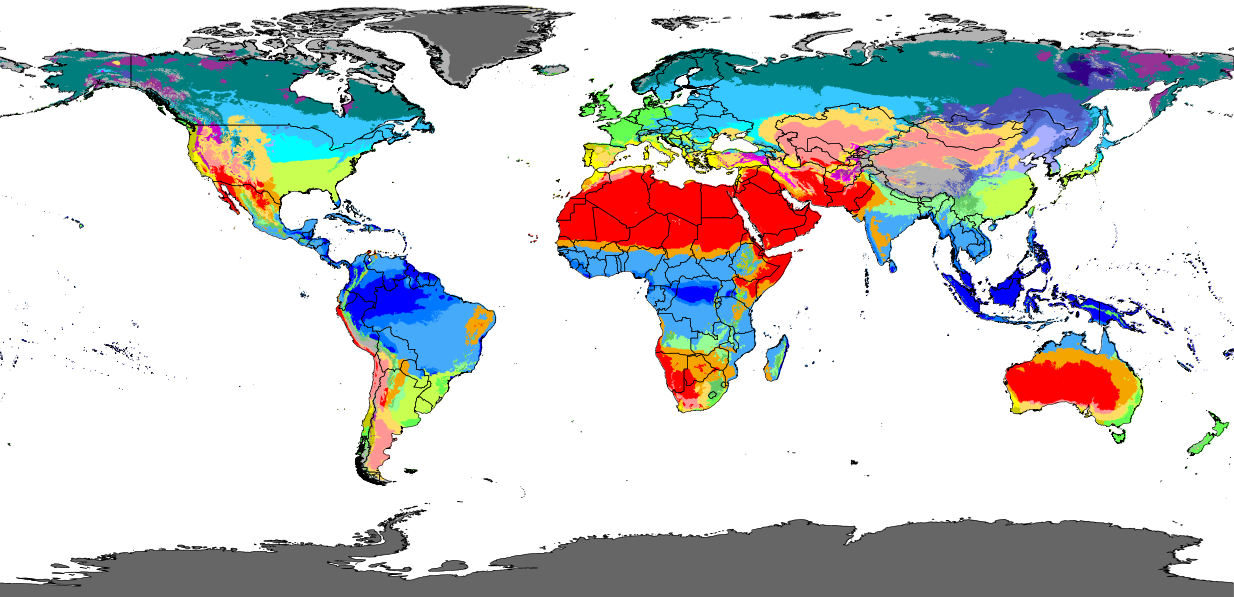
\includegraphics[height=0.3\BenImgWidth]{figures/dataset/KG_Map_cropped.png}};
        \node[anchor=center, font=\scriptsize] (KGMapCap) at ($(KGMap |- LocCap) + (0,0)$) {\textcolor{gray}{Climate}};
        \draw[thin,dotted] ($(PresenceCap.north west) + (0, 0.05)$) -- ($(KGMap.north east |- PresenceCap.west) + (0.05, 0.05)$) -- ($(ClimateLocationTemplate.south east) + (0.05, -.0)$);

        \node[single arrow,minimum height=12mm, minimum width=8mm, single arrow head extend=2mm,
            anchor=west, rotate=90, fill=cyan!90, opacity=0.5] at ($(refMap.north) + (0,-.3)$) {};
        \node[single arrow,minimum height=12mm, minimum width=8mm, single arrow head extend=2mm,
            anchor=west, rotate=0, fill=cyan!90, opacity=0.5] at ($(refMap.east) + (-.3,.4)$) {};
        \node[single arrow,minimum height=12mm, minimum width=8mm, single arrow head extend=2mm,
            anchor=west, rotate=-90, fill=cyan!90, opacity=0.5] at ($(refMap.south) + (0,.3)$) {};
        \node[single arrow,minimum height=10mm, minimum width=8mm, single arrow head extend=2mm,
            anchor=west, rotate=180, fill=cyan!90, opacity=0.5] at ($(refMap.west) + (.3,.4)$) {};

        \node[draw, rounded corners=2mm, thick, dotted, inner sep=4pt, fit=(ClimateLocationTemplate)(SizeCountTemplate), gray!70] (box1) {};

        \node[align=center, anchor=north, text width=99mm, font=\scriptsize] (CombinedTemplates)
            at ($(box1.south) + (0,-0.05)$)
            {
                \colorbox{cyan!20}{This image primary ...  (\textbf{[size]}).}
                \colorbox{WildStrawberry!20}{\textbf{[Class]} is distributed ...  marginal.}
                \colorbox{Dandelion!20}{\textbf{[Class]} is adjacent ... \textbf{[class]}.}
                \colorbox{LimeGreen!20}{The image was ... \textbf{[climate zone]}.}
            };
        \node[draw, rounded corners=2mm, thick, dotted, inner sep=-1pt, fit=(CombinedTemplates), gray!70] (CombinedTemplatesBox) {};
        \node[draw, rounded corners=2mm, thin, dashed, inner sep=1pt, fit=(CombinedTemplatesBox)(box1), gray!90] (TemplatesBox) {};
        \node[inner sep=0pt,minimum size=0pt] (CombineAnchor) at ($(box1.north)!0.5!(CombinedTemplatesBox.south)$) {};
        \node[anchor=center,gray!90, rotate=90, font=\normalsize] at ($(CaptionAnchor |- TemplatesBox)$){\textcolor{gray!90}{\makecell{Extract Attributes,\\Fill \& Concatenate Templates}}};


        \def\scaleLLMRing{0.4}
        \def\LLMRingPointSize{0.05cm}
        \node (baseline_step2_1) at ($(CombinedTemplates.south) + (0,-0.65)$) {};
        \node[anchor=center, draw, circle, minimum size=0.5cm, inner sep=1.5pt, fill=gray!25, font=\tiny] (LLM_paraphrase) at ($(baseline_step2_1) + (-4.15, 0)$) {\scalebox{0.8}{LLM}};
        \node[draw, circle, minimum size=\LLMRingPointSize, inner sep=0pt] (LLM_paraphrase_west) at ($(LLM_paraphrase) + (-\scaleLLMRing,0)$) {};
        \node[draw, circle, minimum size=\LLMRingPointSize, inner sep=0pt] (LLM_paraphrase_east) at ($(LLM_paraphrase) + ( \scaleLLMRing,0)$) {};
        \node[draw, circle, minimum size=\LLMRingPointSize, inner sep=0pt] (LLM_paraphrase_south) at ($(LLM_paraphrase) + (0,-\scaleLLMRing)$) {};
        \node[draw, circle, minimum size=\LLMRingPointSize, inner sep=0pt] (LLM_paraphrase_north) at ($(LLM_paraphrase) + (0, \scaleLLMRing)$) {};
        \node[draw, circle, minimum size=\LLMRingPointSize, inner sep=0pt, fill=black] at ($(LLM_paraphrase) + (-.7070*\scaleLLMRing, .7070*\scaleLLMRing)$) {};
        \node[draw, circle, minimum size=\LLMRingPointSize, inner sep=0pt, fill=black] at ($(LLM_paraphrase) + (-.7070*\scaleLLMRing, -.7070*\scaleLLMRing)$) {};
        \node[draw, circle, minimum size=\LLMRingPointSize, inner sep=0pt, fill=black] at ($(LLM_paraphrase) + (.7070*\scaleLLMRing, .7070*\scaleLLMRing)$) {};
        \node[draw, circle, minimum size=\LLMRingPointSize, inner sep=0pt, fill=black] at ($(LLM_paraphrase) + (.7070*\scaleLLMRing, -.7070*\scaleLLMRing)$) {};
        \centerarc[draw](LLM_paraphrase)(15:30:\scaleLLMRing)
        \centerarc[draw](LLM_paraphrase)(60:75:\scaleLLMRing)
        \centerarc[draw](LLM_paraphrase)(105:120:\scaleLLMRing)
        \centerarc[draw](LLM_paraphrase)(150:165:\scaleLLMRing)
        \centerarc[draw](LLM_paraphrase)(-15:-30:\scaleLLMRing)
        \centerarc[draw](LLM_paraphrase)(-60:-75:\scaleLLMRing)
        \centerarc[draw](LLM_paraphrase)(-105:-120:\scaleLLMRing)
        \centerarc[draw](LLM_paraphrase)(-150:-165:\scaleLLMRing)
        \node[align=justify, anchor=west, text width=80mm, font=\scriptsize] (ParaphrasePrompt)
            at ($(LLM_paraphrase_east.east) + (.1,0)$)
            {\textit{You are a Remote Sensing expert. Use the following definitions to increase variance in the output: ... \\
            Do not violate these rules: ...}};
        \node[draw, rounded corners=2mm, thin, dashed, inner sep=4pt, inner ysep=2pt, fit=(LLM_paraphrase_west)(LLM_paraphrase_north)(LLM_paraphrase_south)(ParaphrasePrompt), gray!90] (box2_1) {};
        \node[anchor=center, gray!90, rotate=90, font=\normalsize] at ($(CaptionAnchor |- box2_1)$) {\textcolor{gray!90}{\makecell{Para-\\phrase}}};

        \node[anchor=center, draw, circle, minimum size=0.5cm, inner sep=1.5pt, fill=gray!25, font=\tiny] (LLM_refine) at ($(LLM_paraphrase) + (0, -1.1)$) {\scalebox{0.8}{LLM}};
        \node[draw, circle, minimum size=\LLMRingPointSize, inner sep=0pt] (LLM_refine_west) at ($(LLM_refine) + (-\scaleLLMRing,0)$) {};
        \node[draw, circle, minimum size=\LLMRingPointSize, inner sep=0pt] (LLM_refine_east)at ($(LLM_refine) + ( \scaleLLMRing,0)$) {};
        \node[draw, circle, minimum size=\LLMRingPointSize, inner sep=0pt] (LLM_refine_south) at ($(LLM_refine) + (0,-\scaleLLMRing)$) {};
        \node[draw, circle, minimum size=\LLMRingPointSize, inner sep=0pt] (LLM_refine_north) at ($(LLM_refine) + (0, \scaleLLMRing)$) {};
        \node[draw, circle, minimum size=\LLMRingPointSize, inner sep=0pt, fill=black] at ($(LLM_refine) + (-.7070*\scaleLLMRing, .7070*\scaleLLMRing)$) {};
        \node[draw, circle, minimum size=\LLMRingPointSize, inner sep=0pt, fill=black] at ($(LLM_refine) + (-.7070*\scaleLLMRing, -.7070*\scaleLLMRing)$) {};
        \node[draw, circle, minimum size=\LLMRingPointSize, inner sep=0pt, fill=black] at ($(LLM_refine) + (.7070*\scaleLLMRing, .7070*\scaleLLMRing)$) {};
        \node[draw, circle, minimum size=\LLMRingPointSize, inner sep=0pt, fill=black] at ($(LLM_refine) + (.7070*\scaleLLMRing, -.7070*\scaleLLMRing)$) {};
        \centerarc[draw](LLM_refine)(15:30:\scaleLLMRing)
        \centerarc[draw](LLM_refine)(60:75:\scaleLLMRing)
        \centerarc[draw](LLM_refine)(105:120:\scaleLLMRing)
        \centerarc[draw](LLM_refine)(150:165:\scaleLLMRing)
        \centerarc[draw](LLM_refine)(-15:-30:\scaleLLMRing)
        \centerarc[draw](LLM_refine)(-60:-75:\scaleLLMRing)
        \centerarc[draw](LLM_refine)(-105:-120:\scaleLLMRing)
        \centerarc[draw](LLM_refine)(-150:-165:\scaleLLMRing)
        \node[align=justify, anchor=west, text width=80mm, font=\scriptsize] (RefinePrompt)
            at ($(LLM_refine_east.east) + (.1,0)$)
            {\textit{Control your caption. Ensure that you followed the rules. Update the caption by ... Do NOT explain the mistakes.}};
        \node[draw, rounded corners=2mm, thin, dashed, inner sep=4pt, inner ysep=2pt, fit=(LLM_refine_west)(LLM_refine_north)(LLM_refine_south)(RefinePrompt), gray!90] (box2_2) {};
        \node[anchor=center,gray!90, rotate=90, font=\normalsize] at ($(CaptionAnchor |- box2_2)$) {\textcolor{gray!90}{\makecell{Refine}}};



        \node[align=justify, anchor=north, text width=108mm, inner sep=2pt, font=\scriptsize] (FinalCaption)
            at ($(box2_2.south) + (0,-0.1)$)
            {This satellite image, captured during the summer season in Switzerland, showcases a diverse landscape within the "temperate, no dry season, warm summer" climate zone. The dominant features are arable land ($\sim$526,000 sqm) and inland wetlands ($\sim$460,000 sqm), which are adjacent to each other. The arable land borders both inland wetlands and urban fabric ($\sim$149,000 sqm). Moreover, the inland wetlands are adjacent to both inland waters ($\sim$305,000 sqm) and urban fabric. Notably, the urban fabric is distributed over three individual marginal areas. The varied landscape presents a mix of agricultural areas, wetlands, water bodies, and artificial surfaces.};
        \node[draw, rounded corners=2mm, thin, dashed, inner sep=0pt, fit=(FinalCaption)($(box2_2.east |- FinalCaption)$)($(box2_2.west |- FinalCaption)$), gray!90] (box3) {};
        \node[anchor=center,gray!90, rotate=90,font=\normalsize] at ($(CaptionAnchor |- box3)$) {\textcolor{gray!90}{\makecell{Final\\Caption}}};

    \end{tikzpicture} 

    \caption{Caption generation process for \bentxt{}: i) Attribute extraction from the reference map and template filling based on the attributes and metadata such as location, season and climate zone information, followed by concatenation of the templates; ii) increasing linguistic variance and ensuring correctness via self-refinement.}
    \label{fig:caption_generation_process}
\end{figure*}
\paragraph{VQA and \genDet{} generation.} We further augment each image pair with question-answer annotations relevant for binary yes/no \ac{VQA}, \ac{MCQ} \ac{VQA}, and \genDet. 
Binary questions target the four spatial categories from the captioning stage (presence, count, size, adjacency), with one \enquote{yes} and one \enquote{no} answer generated per pair. 
To prevent \enquote{no} answers from being solvable by class-absence detection alone, count and size questions are constructed such that the queried class is present but the stated quantity is incorrect; presence and adjacency \enquote{no} questions use semantically similar classes from the \ac{CLC} hierarchy. 
\Acp{MCQ} extend the four spatial categories from the captioning stage with questions about relative class position, acquisition country, season, and Köppen-Geiger climate zone.
Each set of answers for the \acp{MCQ} includes one correct answer and three incorrect ones, sampled by analogous principles to the binary \acp{VQA}. 
For \genDet, we generate \refDet{} instructions targeting instances covering between \SI{1}{\percent} and \SI{50}{\percent} of the image area and at least \SI{40}{\percent} of their enclosing bounding box, along with \pointDet{} instructions for instances whose centroid lies within the instance region. 
Examples are given in \cref{fig:dataset_overview}.
Each annotation type uses more than 20 linguistic templates to ensure variability without relying on \ac{LLM} augmentation. 
In total, each image pair is associated with up to 16 \ac{VQA} pairs, and approximately \SI{80}{\percent} of pairs carry at least one \genDet{} annotation.

\subsection{Caption Statistics\label{sec:statistics}}
The caption annotations of \bentxt{} contain approximately \num{50} million words and \num{2.1} million sentences, averaging 107 words and \num{4.5} sentences. 
The vocabulary comprises \num{12394} unique terms. 
Caption lengths follow a bimodal distribution (\cref{fig:pdf_caption_length}) corresponding to single-class and multi-class scenes: single-class captions are shorter due to the absence of adjacency descriptions, while multi-class captions vary with scene complexity. 
Sentence counts per caption (\cref{fig:pdf_sentences_per_caption}) peak between four and six, reflecting the predominance of complex scenes. 
As shown in \cref{fig:mtld_score}, the caption annotations of \bentxt{} achieve a \ac{MTLD} score of \num{64.69}, surpassing the largest existing image-text \ac{RS} dataset containing images with more than three bands (MS-CLIP~\cite{marimo2025beyond}) by more than $1.7\times$. 
Additionally, caption annotations of \bentxt{} encompass $\sim$\SI{25}{\percent} more words in half as many samples compared to MS-CLIP. This shows that \bentxt{} is not only lexically more diverse, but also richer in the semantic content per caption.
\begin{figure}[h!tb]
\centering
    \subfloat[\notsotiny Length ($\nicefrac{\text{Words}}{\text{Caption}}$)]{
        \raisebox{0mm}{\rotatebox{90}{\hspace{3mm}\textsf{\notsotiny Density of Occurrences}}}
        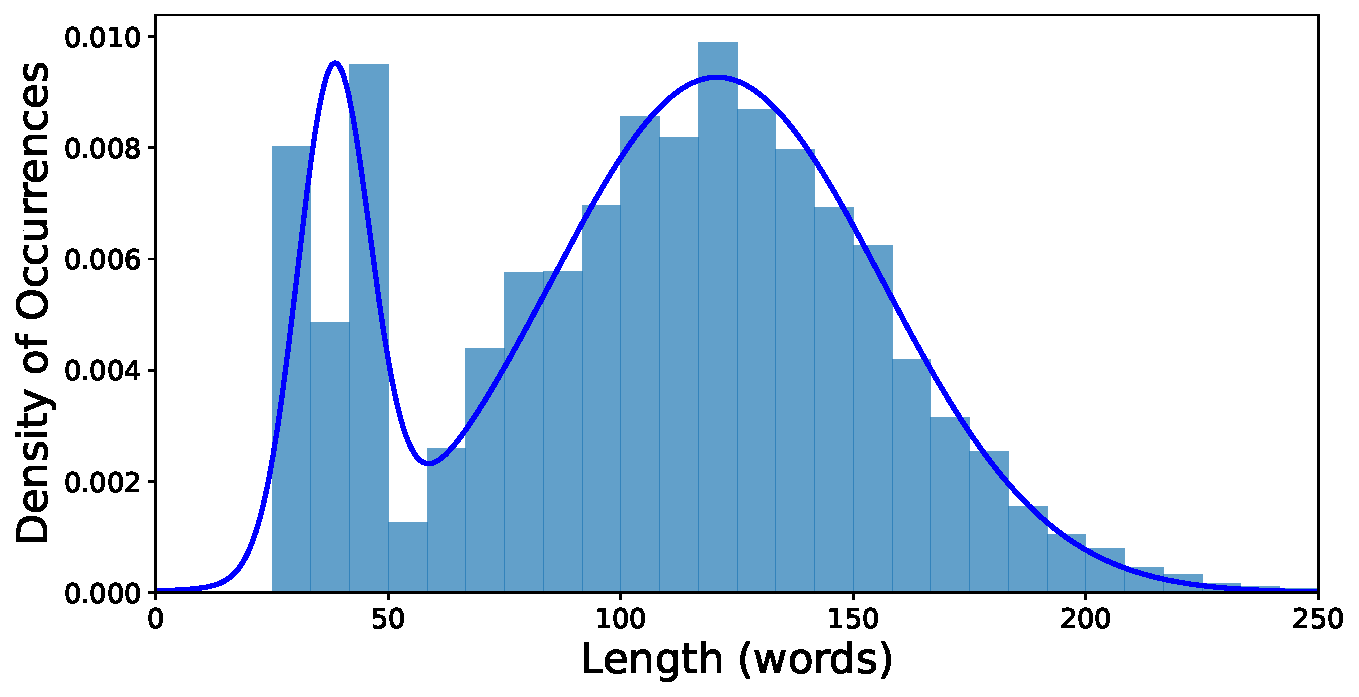
\includegraphics[width=0.44\linewidth,trim=30 32 0 0, clip]{figures/dataset/caption_length_caption_index_2_density.pdf}
        \label{fig:pdf_caption_length}
    }\hfill
    \subfloat[\notsotiny Length ($\nicefrac{\text{Sentences}}{\text{Caption}}$)]{
        \raisebox{0mm}{\rotatebox{90}{\hspace{3mm}\textsf{\notsotiny Density of Occurrences}}}
        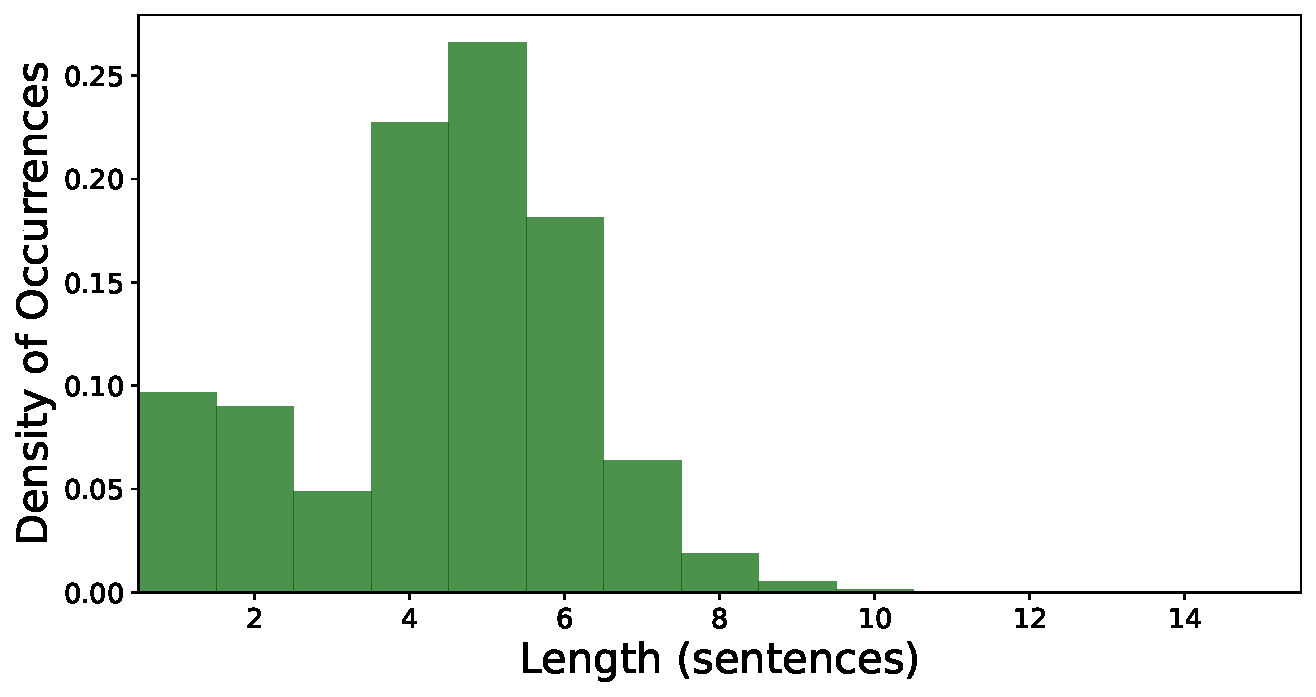
\includegraphics[width=0.44\linewidth,trim=30 32 0 0, clip]{figures/dataset/caption_num_sentences_index_2_density.pdf}
        \label{fig:pdf_sentences_per_caption}
    }\par 
    \subfloat[Number of Image-Text Pairs]{
        \raisebox{0mm}{\rotatebox{90}{\hspace{10mm}\textsf{MTLD Score}}}
        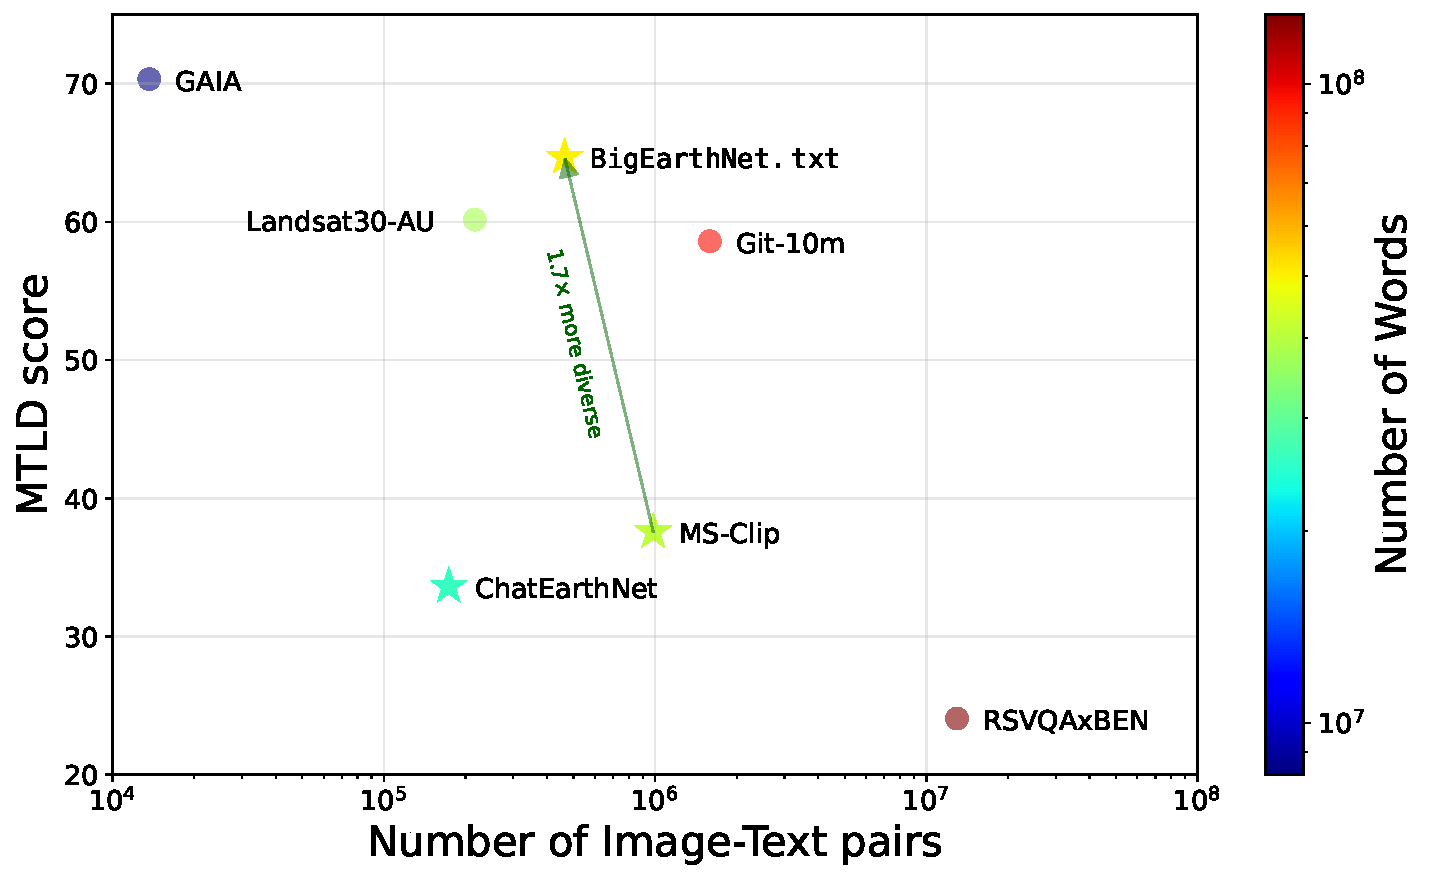
\includegraphics[width=0.45\linewidth,trim=30 30 30 0, clip]{figures/dataset/mtld_score_index_2.pdf}
        \raisebox{0mm}{\rotatebox{90}{\hspace{8mm}\textsf{Number of Words}}}
    \label{fig:mtld_score}
    }
    \caption{\Ac{PDF} of (a) caption lengths and (b) number of sentences in a caption in the \bentxt{} dataset.
     (c) Comparison of existing image-text \ac{RS} datasets in terms of size and semantic richness of the text data. The \ac{NLTK} word tokenizer is used to divide the captions and questions into tokens. The color of each point indicates the total number of tokens in the dataset. Datasets that encompass images with more than three spectral bands are denoted with a star. The \bentxt{} dataset is $1.7\times$ more diverse compared to the largest existing \ac{RS} dataset encompassing more than three bands.}
    \label{fig}
\end{figure}

\subsection{The \bentxt{} \bench{}}

We divide \bentxt{} into train, validation, and test splits as in BigEarthNet~v2.0, resulting in \num{229114}, \num{118095}, and \num{116835} image pairs and \num{4674281}, \num{2454690}, and \num{2424991} text annotations, respectively. However, because LLM-augmented captions may contain hallucinated content, we construct a curated \bench{} to enable reliable model evaluation on the annotations introduced in \bentxt{}. The \bench{} contains \num{1082} image pairs with \num{15029} text annotations from the test split whose augmented captions passed manual verification on all four quality dimensions.
To expose answer-bias in evaluated models, binary and \ac{MCQ} annotations are balanced across answer options.
Annotations are further balanced across \ac{LULC} classes to the extent permitted by their natural distribution. 
Overall, the \bench{} contains \num{6927} binary and \num{5550} multiple-choice \ac{VQA} annotations, \num{970} captions, and \num{1582} \genDet{} annotations across \num{1082} image pairs.

% \section{Multi-Sensor InternVL}
% \label{sec:locationVLM}
% \input{sec/4_vlm}

\section{Experiments}
\label{sec:experiments}
\subsection{Performance Evaluation of VLMs for RS Tasks}
To benchmark \bentxt{} we have considered a wide range of general-purpose \ac{CV} and specialized \ac{RS} \acp{VLM}. In detail, we select five \ac{SOTA} models each from the \ac{CV} and \ac{RS} domain. For the \ac{CV} domain, we select GPT-5.2~\cite{openai2025gpt5}\footnote{OpenAI API, endpoint /v1/chat/completions}, Qwen3-VL~\cite{bai2025qwen3}, GLM-4.6v-Flash~\cite{hong2025glm}, LLaVa-OneVision~\cite{li2024llavaonevision}, and InternVL3-1B~\cite{zhu2025internvl3}, denoted as \gptABBRns, \qwenABBRns, \glmABBRns, \llavaABBRns, and \internvlABBRns, respectively. For the \ac{RS} domain, we select GeoChat~\cite{kuckreja2024geochat}, LHRS-Bot~\cite{muhtar2024lhrs}, SkyEyeGPT~\cite{zhan2025skyeyegpt}, EarthDial~\cite{soni2025earthdial}, and EarthMind~\cite{shu2025earthmind}, denoted as \geochatABBRns, \lhrsbotABBRns, \skyeyegptABBRns, \earthdialrgbABBRns/\earthdialmsABBRns, and \earthmindrgbABBRns/\earthmindsarmsABBRns, respectively.
The majority of these models accept only \ac{RGB} inputs; for these, we provide only the \ac{RGB} bands of \ac{S2} during inference.
As EarthDial and EarthMind also accept multispectral and multi-sensor inputs, we evaluate each under two configurations:
i) \earthdialrgbABBRns{} and \earthmindrgbABBRns{} using \ac{RGB} inputs; and
ii) \earthdialmsABBRns{} and \earthmindsarmsABBRns{} using 12 \ac{S2} bands and \ac{S1}+12 \ac{S2} bands as input, respectively.
We provide the \bentxt{} instructions by default, with additional instructions to follow the output format and model specific tokens where necessary. 
We extract answers even when they do not adhere exactly to the specified format. 
To reduce computational resources during evaluation, we disable thinking for \glmABBRns.
Throughout the paper, we report the results on the \bench{} only.

\cref{tab:main} shows the results obtained for each of our general categories: captioning, binary \ac{VQA}, \ac{MCQ}, and \genDet{}, grouped by \ac{RS} specialized \acp{VLM} (top) and general-purpose \ac{CV} \acp{VLM} (bottom).
From the table, one can observe that none of the \acp{VLM} in general provides good performance, while \ac{CV} \acp{VLM} perform better than \ac{RS} \acp{VLM} in general despite processing only \ac{RGB} input.
This is because \ac{CV} \acp{VLM} exhibit stronger generalizability and instruction-following ability (Tab.~\ref{tab:binary_results}--\ref{tab:bb_point_results}), whereas most \ac{RS} \acp{VLM} are mainly suitable for tasks achievable using solely \ac{RGB} data.
% All checked except Captioning
% Fill TBD values
\begin{table}[h!bt]
    \centering
    \renewcommand{\arraystretch}{\arrayStretchFactor}
    % \footnotesize
    \caption{Results of \ac{VLM}s in \ac{RS} and \ac{CV} on the main categories of the \bentxt{} benchmark split. Reported metrics for captioning: BLEU-4, binary \ac{VQA}: accuracy, \ac{MCQ}: accuracy, and \genDet: \ac{mIoU}. All results in percent (\%). *: Reported parameter count.}
    \begin{tabular}{l c *6{S[table-format=2.2]}}
        \toprule{Model}
        & {\# Parameters}
        & {\makecell{Captioning}}
        & {\makecell{Binary\\VQA}}
        & {\makecell{MCQ}}
        & {\makecell{Ref. Exp.\\Detection}} % Formula for calculation: ref * 0.5019 + point * 0.4981
        \\
        \midrule
        % GeoChat      & 0.81 & 51.31 &  6.37 & 28.13 \\ NO AREA PROMPT
        \geochatABBR & 7B & 0.75 & 50.82 & 28.36 & 4.85 \\ % 4.36 if non-rotated BBs are taken
        % LHRS-Bot     & 0.61 & 47.91 & 5.18 & 23.30 \\ NO AREA PROMPT
        \lhrsbotABBR  & 7B & 0.43 & 48.23 & 22.99 & 4.79 \\
        \skyeyegptABBR & 7B & 0.00 & 48.87 & 27.60 & 6.08 \\
        \earthdialrgbABBR & 4B & 0.62 & 58.38 & 32.94 & 7.13 \\ % 6.79 if non-rotated BBs are taken
        \earthdialmsABBR & 4B & 0.00 & 44.06 & 8.43 & 0.49 \\
        \earthmindrgbABBR & 4B & \best{1.66} & 57.90 & 34.25 & 12.12 \\
        % EarthMind~\cite{shu2025earthmind} & \earthmindmsABBR & S2 & 4B & {TBD} & {TBD} & {TBD} & {TBD} \\
        \earthmindsarmsABBR & 4B & \second{1.46} & 57.79 & 35.26 & 16.18 \\
        \midrule
        \gptABBR & 2T* & 0.30 & \second{60.39} & 34.93 & \best{31.73} \\
        % Qwen3-VL & 0.69 & 61.99 & 16.79 & 38.29 \\ NO AREA PROMPT
        \qwenABBR & 8B & 0.57 & \best{61.96} & \best{37.55} & 18.00 \\
        % GLM-4.6v-Flash & 0.62 & 53.47 & 20.27 & 34.65 \\ NO AREA PROMPT
        \glmABBR & 10B & 0.79 & 56.59 & 34.45 & \second{27.24} \\
        % LLaVa-OV & 1.11 & 59.07 & 21.98 & 36.54 \\ NO AREA PROMPT
        \llavaABBR & 7B & 0.96 & 58.60 & \second{36.27} & 20.17 \\
        \internvlABBR & 1B & 0.45 & 54.11 & 26.76 & 5.76 \\
        % InternVL-3 (8B) & 0.72 & {--} & 10.12 & {--} \\
        % \midrule
        % \textbf{RS-InternVL~(ours)} & \internvlrsABBR & S1, S2 & 1B & \best{34.04} & \best{73.29} & \best{65.84} & \best{51.49} \\
        % Rebalanced-RSInternVL & 34.04 & 67.31 & 25.17 & 65.84 \\
        \bottomrule
    \end{tabular}
    \label{tab:main}
\end{table}
The considered \ac{CV} \acp{VLM} may also have been pretrained using some \ac{RS} data, which is a growing trend in recent works~\cite{simeoni2025dinov3}.
Additionally, models accepting multispectral (\earthdialmsABBRns) or multi-sensor (\earthmindsarmsABBRns) inputs show no consistent benefit (and in some cases decreased performance) compared to their \ac{RGB} counterparts.
This is because their pre-training and fine-tuning data largely consist of \ac{RGB} images, and the models were therefore not trained to exploit the additional spectral information provided at inference.
Even \gptABBR{}, which is the largest model, scores only 60.39\% on binary \ac{VQA} and 34.93\% on \ac{MCQ} due to its inherent \ac{RGB} data limitation.
\cref{tab:binary_results} shows detailed per-task results for binary \ac{VQA}.
From the table, one can clearly observe that for some tasks, models perform noticeably better (\eg, \SI{69.34}{\percent} accuracy for EarthMind on the binary \emph{presence} task).
% All checked
% Area prompt for area questions included
% Counted unexpected answers as incorrect
\begin{table}[tb]
    \centering
    \renewcommand{\arraystretch}{\arrayStretchFactor}
    \caption{Results on the binary VQA tasks for \ac{VLM}s in \ac{RS} and \ac{CV}: Presence, Area, Counting, Adjacency, and Overall, denoted as \presenceABBR, \areaABBR, \countABBR, \adjacencyABBR, and \overallABBR, in terms of accuracy. All results are in percent (\%). \instructionfollowedABBR\ shows whether an unambiguous answer could be extracted all the time.}
    \begin{tabular}{l *5{S[table-format=2.2]} *1{S[table-format=3.2]}}
        \toprule
        {\thead{Model}}
        & {\presenceABBR}
        & {\areaABBR}
        & {\countABBR}
        & {\adjacencyABBR}
        & {\overallABBR}
        & {\instructionfollowedABBR} % Idea: Maybe give the percentage of followed instructions, 6927 binary samples
        \\
        \midrule
        % GeoChat & 51.65 & 49.46 & 43.57 & 55.51 & 51.31 & \bfseries 0 \\ NO AREA PROMPT
        \geochatABBR & 51.65 & 46.86 & 43.57 & 55.51 & 50.82 & \gcmark \\
        % LHRS-Bot & 48.83 & 49.54 & 49.23 & 46.10 & 47.91 & 51 \\ NO AREA PROMPT
        \lhrsbotABBR & 48.83 & 51.23 & 49.23 & 46.10 & 48.23 & \rxmark \\ % 38
        % SkyEyeGPT & 51.51 & 52.07 & 45.71 & 46.83 & 48.59 & \bfseries 0 \\
        \skyeyegptABBR & 52.19 & 51.61 & 46.63 & 46.94 & 48.87 & \gcmark \\
        %ED\textsubscript{RGB} & 65.10 & 53.14 & 51.99 & 60.62 & 58.51 & 14 \\
        \earthdialrgbABBR & 64.47 & 53.06 & 51.99 & \best{60.62} & 58.38 & \rxmark \\ % 14
        % ED\textsubscript{MS} & 56.99 & 58.99 & 53.61 & 54.53 & 55.49 & 1427 \\ % With area prompt
        \earthdialmsABBR & 37.45 & 40.20 & 47.17 & 47.78 & 44.06 & \rxmark \\ % 1427
        \earthmindrgbABBR & \best{69.34} & 56.20 & 51.07 & 55.97 & 57.90 & \gcmark \\
        \earthmindsarmsABBR & \second{69.07} & 54.59 & 50.15 & 56.98 & 57.79 & \gcmark \\
        \midrule
        \gptABBR & 61.59 & \best{67.38} & \second{61.94} & 55.86 & \second{60.39} & \gcmark \\
        %Qwen & 63.37 & 68.07 & 61.64 & 58.66 & 61.99 & 0 \\
        \qwenABBR & 64.33 & \second{66.62} & \best{62.33} & 58.45 & \best{61.96} & \gcmark \\
        % GLM & 60.01 & 64.40 & 54.75 & 53.03 & 56.97 & \bfseries 0 \\ NO AREA PROMPT
        \glmABBR & 60.01 & 62.40 & 54.75 & 53.03 & 56.59 & \gcmark \\
        % LLaVa & 62.07 & 60.72 & 54.36 & 58.94 & 59.07 & \bfseries 0 \\ NO AREA PROMPT
        \llavaABBR & 62.07 & 58.19 & 54.36 & \second{58.94} & 58.60 & \gcmark \\ 
        % InternVL & 58.09 & 50.80 & 53.52 & 55.01 & 54.58 & 2 \\ NO AREA PROMPT
        % InternVL (1B) & 57.27 & 47.55 & 50.34 & 55.39 & 53.36 & 2 \\
        \internvlABBR & 56.24 & 48.77 & 51.61 & 56.60 & 54.11 & \rxmark \\
        % \midrule
        % \textbf{\internvlrsABBR} & \best{69.68} & \best{82.39} & \best{78.02} & \best{68.81} & \best{73.29} & \gcmark \\
        % Rebalanced-RSInternVL & 64.76 & 74.96 & 70.72 & 63.54 & 67.13 & 228 \\
        \bottomrule
        \end{tabular}
    \label{tab:binary_results}
\end{table}
This good result on presence \ac{VQA} is expected, as determining whether a \ac{LULC} class appears in an image is closely analogous to scene classification, which is a dominant objective in \ac{RS} \ac{VLM} pre-training datasets~\cite{kuckreja2024geochat, muhtar2024lhrs, zhan2025skyeyegpt, soni2025earthdial, shu2025earthmind, hu2025rsgpt}.
Nevertheless, none of these models, including the largest, \gptABBRns, achieve consistently strong performance across all binary \ac{VQA} tasks.
In \cref{tab:mcq_results}, one can observe the performance on the \ac{MCQ} tasks.
% All checked
% Area prompt for area questions included
% Counted unexpected answers as incorrect
\begin{table}[h!bt]
    \centering
    \renewcommand{\arraystretch}{\arrayStretchFactor}
    %\setlength{\tabcolsep}{1.4pt}
    \caption{Results on the \ac{MCQ} tasks for \ac{VLM}s in \ac{RS} and \ac{CV}: Presence, Area, Counting, Adjacency, Relative Position, Country, Season, Climate Zone, and Overall, denoted as \presenceABBR, \areaABBR, \countABBR, \adjacencyABBR, \relativepositionABBR, \countryABBR, \seasonABBR, \climateABBR, and \overallABBR, respectively in terms of accuracy. All results are in percent (\%). \instructionfollowedABBR\ shows whether an unambiguous answer could be extracted all the time.}
    \begin{tabular}{l *9{S[table-format=2.2]} *1{S[table-format=3.2]}}
    \toprule
    Model
    & {\presenceABBR}
    & {\areaABBR}
    & {\countABBR}
    & {\adjacencyABBR}
    & {\relativepositionABBR}
    & {\countryABBR}
    & {\seasonABBR}
    & {\climateABBR}
    & {\overallABBR}
    & {\instructionfollowedABBR} \\ % Idea: Maybe give the percentage of followed instructions, 5550 MCQ samples
    \midrule
        % GeoChat & 32.63 & 25.88 & 24.72 & 29.93 & 34.62 & 22.57 & 30.52 & 28.17 & 9 \\
        % GeoChat & 32.58 & 25.88 & 24.72 & 29.75 & 25.46 & 34.62 & 22.57 & 30.52 & 28.13 & 9 \\ NO AREA PROMPT
        \geochatABBR & 32.58 & 26.80 & 24.72 & 29.75 & 25.46 & 34.62 & 22.57 & 30.52 & 28.23 & \rxmark \\ % 9
        % LHRS-Bot & 23.97 & 20.83 & 22.66 & 27.44 & 17.54 & 29.08 & 24.52 & 23.87 & 134 \\
        % LHRS-Bot & 23.84 & 19.14 & 21.19 & 27.23 & 17.48 & 17.48 & 28.53 & 23.71 & 23.30 & 134 \\ NO AREA PROMPT
        \lhrsbotABBR & 23.84 & 16.54 & 21.19 & 27.23 & 17.48 & 28.53 & 23.71 & 23.56 & 22.99 & \rxmark \\ % 295
        % SkyEyeGPT & 30.47 & 17.76 & 24.91 & 30.89 & 23.62 & 23.62 & 28.85 & 25.29 & 27.30 & \best{ 0 \\
        \skyeyegptABBR & 30.89 & 21.75 & 24.91 & 30.51 & 22.09 & 29.81 & 24.71 & 33.63 & 27.60 & \gcmark \\
        % ED\textsubscript{RGB} & 57.82 & 27.62 & 36.43 & 47.07 & 54.17 & 25.57 & 31.03 & 37.57 & 685 \\ % with area prompt
        \earthdialrgbABBR & \best{46.40} & 27.41 & \best{36.43} & 30.66 & 29.14 & \best{54.17} & 25.57 & 27.26 & 32.94 & \rxmark \\ % 685 % with area prompt, unexpected as incorrect
        % ED\textsubscript{MS} & 28.79 & 25.53 & 24.51 & 26.53 & 32.41 & 29.09 & 28.49 & 27.99 & \color{red} 3878 \\
        \earthdialmsABBR & 21.16 & 5.51 & 4.65 & 8.62 & 0.00 & 15.06 & 6.86 & 7.26 & 8.43 & \rxmark \\ % 3878
        \earthmindrgbABBR & 41.75 & 24.81 & 27.32 & 42.87 & 29.91 & 40.06 & 23.43 & 37.04 & 34.25 & \rxmark \\ % 334
        \earthmindsarmsABBR & \second{43.58} & 25.57 & 25.28 & \best{44.70} & 31.60 & 40.06 & 25.71 & 36.74 & 35.26 & \rxmark \\ % 383 
        \midrule
        \gptABBR & 38.08 & \best{44.41} & 22.68 & 39.16 & 27.91 & 41.35 & 28.43 & 34.52 & 34.93 & \gcmark \\
        % Qwen3-VL & 35.03 & 36.45 & 32.34 & 43.48 & 38.34 & 47.76 & 27.29 & 38.30 & 1 \\
        % Qwen3-VL & 34.98 & 36.45 & 32.34 & 43.48 & 38.34 & 38.34 & 47.76 & 27.29 & 38.29 & 1 \\ NO AREA PROMPT
        \qwenABBR & 34.41 & \second{37.67} & 29.00 & 42.87 & \second{34.66} & \second{47.76} & \second{27.29} & \best{45.93} & \best{37.55} & \gcmark \\
        % GLM-4.6v-Flash & 34.27 & 34.00 & 34.01 & 39.44 & 31.90 & 38.78 & 24.71 & 37.93 & 34.65 & \best{0 \\ NO AREA  PROMPT
        \glmABBR & 34.27 & 32.31 & \second{34.01} & 39.44 & 31.90 & 38.78 & 24.71 & 37.93 & 34.45 & \gcmark \\
        % LLaVA-OV & 34.56 & 34.76 & 32.71 & 43.33 & 34.82 & 40.38 & 27.43 & 39.56 & 36.54 & \best{0 \\ NO AREA PROMPT
        \llavaABBR & 34.56 & 32.47 & 32.71 & \second{43.33} & \best{34.82} & 40.38 & \best{27.43} & \second{39.56} & \second{36.27} & \gcmark \\
        % InternVL-3 (1B) & 31.31 & 24.66 & 24.54 & 29.44 & 25.46 & 29.17 & 23.43 & 28.74 & 27.32 & 189 \\ NO AREA PROMPT
        % InternVL3 (1B) & 28.26 & 26.96 & 26.57 & 29.85 & 26.97 & 29.58 & 23.15 & 27.07 & 27.50 & 131 \\
        \internvlABBR & 28.77 & 26.03 & 23.05 & 30.59 & 23.01 & 26.92 & 24.29 & 26.96 & 26.76 & \rxmark \\
        % \midrule
        % \textbf{\internvlrsABBR} & \best{64.88} & \second{42.11} & \best{55.20} & \best{56.90} & \best{57.98} & \best{88.78} & \best{89.14} & \best{88.44} & \best{65.84} & \gcmark \\
    \bottomrule
    \end{tabular}
    \label{tab:mcq_results}
\end{table}
These results closely mirror the binary \ac{VQA} findings: the best performance is again observed on tasks that most closely resemble typical pre-training objectives.
Beyond understanding the image content, instruction-following is an additional challenge: most \ac{RS} models struggle to consistently adhere to the \ac{MCQ} format, as this task is less common in \ac{RS} \ac{VLM} pre-training data and thus less reliably learned.
The results on \refDet{} and \pointDet{} are presented in \cref{tab:bb_reference_results} and \cref{tab:bb_point_results}.
For models trained on segmentation rather than bounding box prediction, we derive bounding boxes from their segmentation outputs.
In \refDet, models must identify and localize a target instance from a textual description alone, without any spatial prior.
In \pointDet, models are additionally provided with a point within the target instance, and must predict the enclosing bounding box.
As one can see from the table, several models from the \ac{CV} domain perform substantially better on \pointDet{} than on \refDet.
We think that the provided point allows models with strong general spatial reasoning to constrain the predicted box to the vicinity of the given location, reducing the task to local boundary estimation rather than open-vocabulary instance search.
GPT achieves the best performance on both task types, mainly owing to its scale and the breadth of its pre-training data.
% All checked
% Counted unexpected answers with IoU = 0.0
\begin{table}[h!bt]
    \centering
    \renewcommand{\arraystretch}{\arrayStretchFactor}
    % \scriptsize
    % \setlength{\tabcolsep}{1pt}
    %\caption{Bounding Box Results of RS VLMs for the \textbf{referring expression} task (794 total samples). The subscripts \textit{rect} and \textit{arb} indicate the shape of the convex hull used for the GIoU calculation. The superscript \textit{*} indicates that the output bounding boxes are \textbf{not} rotated. \textsubscript{F.} indicates that the original bench samples are subsampled, to exclude images already seen by the model during training, i.e. earthdial is left with 264 samples.}
    \caption{Results on \refDet{} for \ac{VLM}s in \ac{RS} and \ac{CV} in terms of \ac{mIoU}, and accuracy@$k$ (where a prediction is counted as correct if the overlap with the reference is greater than $k\%$). All results are in percent (\%). \instructionfollowedABBR\ shows whether an unambiguous answer could be extracted all the time.}
    \begin{tabular}{l *5{S[table-format=2.2]} *1{S[table-format=3.2]}}
        \toprule
        {Model} 
        & {mIoU}
        & {Acc@25} 
        & {Acc@50} 
        & {Acc@75} 
        & {Acc@90}
        & {\instructionfollowedABBR} \\ % 794 BBox - reference samples
        \midrule
        % \geochatABBR\textsuperscript{*}    & 6.37 & 8.44 & 1.01 & 0.00 & 0.00 & \gcmark \\ % No rotation
        \geochatABBR   & 7.51 & 11.34 & 1.51 & 0.00 & 0.00 & \gcmark \\ % Rotation
        \lhrsbotABBR   & 7.47 & 12.59 & 1.89 & 0.50 & 0.00 & \rxmark \\
        \skyeyegptABBR & 12.12 & 20.03 & 6.55 & 2.27 & 0.13 & \gcmark \\
        % \earthdialrgbABBR\textsuperscript{*} & 8.29 & 11.84 & 2.52 & 0.13 & 0.00 & \gcmark \\
        % \earthdialrgbABBR   & 7.99 & 10.58 & 2.39 & 0.25 & 0.00 & \gcmark \\
        \earthdialrgbABBR   & 8.99 & 12.85 & 2.02 & 0.00 & 0.00 & \gcmark \\
        % \earthdialmsABBR\textsuperscript{*} & 0.96 & 0.38 & 0.00 & 0.00 & 0.00 & \rxmark \\ % 485
        % \earthdialmsABBR   & 0.96 & 0.38 & 0.00 & 0.00 & 0.00 & \rxmark \\ % 485
        \earthdialmsABBR   & 0.98 & 0.63 & 0.00 & 0.00 & 0.00 & \rxmark \\ % 533 % Calculate over both categories
        % \earthmindrgbABBR   & 14.86 & 24.18 & 11.46 & 4.16 & \second{1.13} & \rxmark \\ % 263
        \earthmindrgbABBR   & 21.90 & 35.52 & \second{17.88} & \best{5.67} & \best{1.39} & \rxmark \\ % 59 
        % \earthmindsarmsABBR & 19.69 & 32.75 & 13.10 & 3.65 & 0.76 & \rxmark \\ % 54 93.20
        \earthmindsarmsABBR & 22.65 & \second{38.41} & 16.62 & \second{4.53} & 1.01 & \rxmark \\ % 35
        % For EarthMind, the model cannot output a BB (it was not trained on BB at all), but it can segment
        % Problem in EarthMind is not instruction following, but the returned segmentation map is empty (or non was outputted)
        \midrule
        % \gptABBR & \best{24.56} & \best{40.81} & \best{17.88} & \best{4.53} & \second{1.13} & \gcmark \\
        \gptABBR & \best{25.16} & \best{40.81} & \best{19.52} & 4.28 & \second{1.26} & \gcmark \\
        \qwenABBR & 15.60 & 25.31 & 9.95 & 2.39 & 0.38 & \gcmark \\
        \glmABBR & 22.35 & 37.03 & 16.75 & 3.53 & \best{1.39} & \gcmark \\
        \llavaABBR & \second{23.04} & \second{38.41} & 15.74 & 3.90 & 0.63 & \gcmark \\
        \internvlABBR & 5.01 & 5.29 & 0.88 & 0.00 & 0.00 & \rxmark \\
        % \midrule
        % \textbf{\internvlrsABBR} & \best{33.16} & \second{47.73} & \best{34.38} & \best{18.77} & \best{6.55} & \gcmark \\
        \bottomrule
    \end{tabular}
    \label{tab:bb_reference_results}
\end{table}
% All checked
% Counted unexpected answers with IoU = 0.0
\begin{table}[h!bt]
    \centering
    \renewcommand{\arraystretch}{\arrayStretchFactor}
    % \scriptsize
    % \setlength{\tabcolsep}{1pt}
    %\caption{Bounding Box Results of RS VLMs for the \textbf{referring expression} task (794 total samples). The subscripts \textit{rect} and \textit{arb} indicate the shape of the convex hull used for the GIoU calculation. The superscript \textit{*} indicates that the output bounding boxes are \textbf{not} rotated. \textsubscript{F.} indicates that the original bench samples are subsampled, to exclude images already seen by the model during training, i.e. earthdial is left with 264 samples.}
    \caption{Results on \pointDet{} for \ac{VLM}s in \ac{RS} and \ac{CV} in terms of \ac{mIoU}, and accuracy@$k$ (where a prediction is counted as correct if the overlap with the reference is greater than $k\%$). \instructionfollowedABBR\ shows whether an unambiguous answer could be extracted all the time.}
    \begin{tabular}{l *5{S[table-format=2.2]} *1{S[table-format=3.2]}}
        \toprule
        {Model} 
        & {mIoU}
        & {Acc@25} 
        & {Acc@50} 
        & {Acc@75} 
        & {Acc@90}
        & {\instructionfollowedABBR} \\ % 788 BBox - point samples
        \midrule
        % GeoChat*    & {--} & {--} & {--} & {--} & {--} & \\
        % GeoChat     & 2.34 & 3.55 & 1.14 & 0.13 & 0.00 & 0 \\
        % \geochatABBR\textsuperscript{*} & 2.34 & 3.55 & 1.14 & 0.13 & 0.00 &  \\ % 658 19.76
        \geochatABBR & 2.16 & 3.43 & 0.63 & 0.13 & 0.00 & \rxmark \\ % 658 19.76
        \lhrsbotABBR & 3.09 & 0.25 & 0.00 & 0.00 & 0.00 & \rxmark \\
        \skyeyegptABBR & 0.00 & 0.00 & 0.00 & 0.00 & 0.00 & \rxmark \\
        % \earthdialrgbABBR\textsuperscript{*} & 5.27 & 3.05 &  0.13 &  0.00 &  0.00 & \best{100.00} \\
        \earthdialrgbABBR & 5.26 & 3.05 &  0.13 &  0.00 &  0.00 & \gcmark \\
        % \earthdialmsABBR\textsuperscript{*} & 0.00 & 0.00 & 0.00 & 0.00 & 0.00 & 0.13 \\ % 787
        \earthdialmsABBR & 0.00 & 0.00 & 0.00 & 0.00 & 0.00 & \rxmark \\ % 0.13
        \earthmindrgbABBR & 9.35 & 14.21 & 4.57 & 1.27 & 0.13 & \rxmark \\ % 249 68.40
        \earthmindsarmsABBR & 12.65 & 17.51 & 5.08 & 0.89 & 0.13 & \rxmark \\
        \midrule
        \gptABBR & \best{38.95} & \best{64.21} & \best{35.53} & \best{8.63} & \best{2.79} & \gcmark \\
        \qwenABBR & 20.42 & 28.81 & 8.25 & 0.89 & 0.00 & \gcmark \\
        \glmABBR & \second{32.16} & \second{56.09} & \second{22.46} & \second{4.82} & \second{1.40} & \gcmark \\
        \llavaABBR & 17.27 & 19.67 & 3.17 & 0.51 & 0.13 & \gcmark \\
        \internvlABBR & 6.52 & 3.05 & 0.00 & 0.00 & 0.00 & \rxmark \\
        % \midrule
        % \textbf{\internvlrsABBR} & \best{69.95} & \best{95.43} & \best{82.23} & \best{48.22} & \best{12.69} & \best{100.00} \\
        \bottomrule
    \end{tabular}
    \label{tab:bb_point_results}
\end{table}
Finally, \cref{tab:captioning} shows the obtained performance on the captioning task across several metrics.
\begin{table}[h!bt]
    \centering
    \renewcommand{\arraystretch}{\arrayStretchFactor}
    
    \caption{Results on the captioning task for \ac{VLM}s in \ac{RS} and \ac{CV} in terms of n-gram-based (BLEU-4, ROUGE, METEOR, CIDEr), sentence-embedding-based (BERTScore, SBert-Cosine) and \ac{LLM}-based (CLAIR) metrics. All results are in percent (\%).}
    \begin{tabular}{l *7{S[table-format=2.2]}}
        \toprule
         Model
         & {BLEU-4}
         & {ROUGE}
         & {METEOR}
         & {CIDEr}
         & {BERTScore}
         & {\makecell{SBERT-\\Cosine}}
         & {CLAIR} \\
         \midrule
         \geochatABBR & 0.75 & 14.95 & 14.24 & 0.65 & 83.42 & 43.05 & 19.91 \\
         \lhrsbotABBR & 0.72 & 12.44 & 16.93 & 0.01 & 82.52 & \second{54.61} & 28.62 \\
         \skyeyegptABBR & 0.00 & 5.91 & 2.21 & 0.00 & 82.79 & 38.30 & 43.86 \\
         \earthdialrgbABBR & 0.48 & 13.65 & 11.36 & 0.51 & 83.45 & 50.49 & 46.51 \\
         \earthdialmsABBR & 0.03 & 8.64 & 3.51 & 0.00 & 83.34 & 35.00 & \best{59.70} \\
         \earthmindrgbABBR & \best{1.66} & \best{16.54} & 14.93 & \best{0.96} & \best{84.34} & 50.55 & 56.73 \\
         \earthmindsarmsABBR & \second{1.46} & \second{16.43} & 14.62 & 0.76 & \second{84.15} & 51.97 & 56.45 \\
         \midrule
         \gptABBR & 0.30 & 13.39 & 12.69 & 0.63 & 83.58 & 52.52 & 57.68 \\
         \qwenABBR & 0.70 & 11.09 & \best{17.83} & 0.01 & 81.87 & 52.62 & 28.38 \\
         \glmABBR & 0.79 & 14.94 & \second{17.05} & 0.43 & 83.51 & \best{55.90} & 50.91 \\
         \llavaABBR & 0.96 & 14.84 & 15.41 & \second{0.81} & 83.89 & 52.39 & \second{58.91} \\
         \internvlABBR & 0.34 & 11.61 & 16.71 & 0.06 & 81.75 & 51.22 & 35.68 \\
         % \midrule
         % \internvlrsABBR & 34.04 & 50.63 & 50.62 & 78.35 & 91.87 & 83.29 & 70.90 \\
         \bottomrule
    \end{tabular}
    \label{tab:captioning}
\end{table}
We employ n-gram-based (BLEU, ROUGE, METEOR, CIDEr), embedding-based (BERTScore, SBERT-Cosine \cite{zhang2019bertscore, reimers-gurevych-2019-sentence}), and \ac{LLM}-based metrics (CLAIR~\cite{chan-etal-2023-clair}).
For CLAIR, an \ac{LLM} is prompted to output a score between 0 and 100 for a candidate caption based on how likely it describes the same image as the reference caption. We use the distilled reasoning model \textit{DeepSeek-R1-Distill-Qwen-32B} with greedy decoding as the judge.
We observe that all evaluated \ac{SOTA} \acp{VLM} have limited capabilities in describing existing \ac{LULC} classes and their spatial composition in detail.

In general, these results demonstrate that \ac{SOTA} \acp{VLM} currently fall short on tasks requiring multi-sensor spectral information and complex \ac{LULC} understanding.
Exceptions arise when a task closely resembles the model's pre-training objectives, \eg, EarthMind's strong performance on binary presence \ac{VQA}.
This suggests that the poor generalization to other \bentxt{} tasks is primarily a consequence of insufficient pre-training data, rather than an inherent limitation of the model architectures themselves.

\subsection{Results of Multi-Sensor InternVL (RS-InternVL)}

%To demonstrate that strong performance on the \bentxt{} \bench{} is achievable given adequate task-relevant training data, 
Using the training and validation sets of \bentxt{}, we fine-tune a \ac{SOTA} \ac{VLM} adapted to accommodate multi-sensor input and evaluate it on the \bench{}. To this end, we build on InternVL-3-1B~\cite{zhu2025internvl3} as a backbone and introduce modality-specific branches for \ac{S1} and \ac{S2} inputs, while we retain the original InternVL components. The architecture is denoted as (\ac{RS}-InternVL). 
For each sensor modality, a pretrained \ac{ViT} produces patch embeddings, which are aligned to the InternVL \ac{LLM} embedding space via linear projection layers.
The projected \ac{S1} and \ac{S2} tokens are concatenated with the \ac{RGB} tokens and the tokenized instruction before being passed to the \ac{LLM}.
To preserve pretrained representations and reduce computational complexity, all \ac{ViT} backbones are frozen. 
Only the modality-specific projections and LoRA adapters for the \ac{LLM} (rank 8, $\alpha=32$, dropout \num{0.1}) are trained, resulting in \SI{5.8}{\mega\nothing} trainable parameters out of \SI{1.1}{\bel\nothing} in total.
We initialize the \ac{S1} and \ac{S2} encoders with BigEarthNet-pretrained \acp{ViT}~\cite{clasen2025reben}, removing their classification heads. 
We process only the \SI{10}{\meter} and \SI{20}{\meter} bands of \ac{S2}, as the \SI{60}{\meter} bands are primarily used for cloud screening and atmospheric correction and carry limited information for semantic \ac{RS} image understanding~\cite{sumbul2021bigearthnet}.
Training uses a linear warm-up cosine annealing schedule, increasing the learning rate from $10^{-6}$ to $10^{-4}$ over the first \SI{1}{\percent} of steps, followed by cosine decay.
We fine-tune separately for each task to provide per-task baselines.
The model is fine-tuned on the combined training and validation sets for one epoch and evaluated on the \bentxt{} \bench{}.
Fine-tuning takes approximately two days on four NVIDIA H200 GPUs in total.

\cref{tab:main_ours} shows the results obtained by RS-InternVL on the general categories.
From the table, one can see that, once a model is fine-tuned on pairs of \ac{S1} and \ac{S2} data with diverse text annotations, performance on the \bench{} improves substantially across all tasks, even at small model scale.
% All checked except Captioning
% Fill TBD values
\begin{table}[h!tb]
    \centering
    \renewcommand{\arraystretch}{\arrayStretchFactor}
    % \footnotesize
    \caption{Results on the main tasks of the \bentxt{} benchmark split for the fine-tuned adapted RS-InternVL model as well as best results from \ac{VLM}s in \ac{RS} and \ac{CV}, which are \earthmindrgbABBR{} and \llavaABBR{} for captioning, \earthdialrgbABBR{} and \qwenABBR{} for binary \ac{VQA}, \earthmindsarmsABBR{} and \qwenABBR{} for \ac{MCQ}, and \earthmindsarmsABBR{} and \gptABBR{} for \genDet. 
    Reported metric for captioning is BLEU-4, while that for binary \ac{VQA}, and \ac{MCQ} is accuracy, and that for \genDet{} is mIoU. All results are in percent (\%).}
    \begin{tabular}{l *5{S[table-format=2.2]}}
        \toprule
        {Model}
        & {\makecell{Captioning}}
        & {\makecell{Binary VQA}}
        & {\makecell{MCQ}} 
        & {\makecell{Ref. Exp.\\Detection}}% Formula for calculation: ref * 0.5019 + point * 0.4981
        \\
        \midrule
        % GeoChat      & 0.81 & 51.31 &  6.37 & 28.13 \\ NO AREA PROMPT
        % GeoChat~\cite{kuckreja2024geochat} & \geochatABBR & $\text{S2}_{RGB}$ & 7B & 0.75 & 50.82 & 4.25 & 28.36 \\ % 4.36 if non-rotated BBs are taken
        % % LHRS-Bot     & 0.61 & 47.91 & 5.18 & 23.30 \\ NO AREA PROMPT
        % LHRS-BOT~\cite{muhtar2024lhrs} & \lhrsbotABBR & RGB  & 7B & 0.43 & 48.23 & 4.14 & 22.99 \\
        % SkyEyeGPT~\cite{zhan2025skyeyegpt} & \skyeyegptABBR & RGB & 7B & 0.00 & 48.87 & 5.92 & 27.60 \\
        % EarthDial~\cite{soni2025earthdial} & \earthdialrgbABBR & RGB & 4B & 0.62 & 58.38 & 6.63 & 32.94 \\ % 6.79 if non-rotated BBs are taken
        % EarthDial~\cite{soni2025earthdial} & \earthdialmsABBR & S2 & 4B & 0.00 & 44.06 & 0.48 & 8.43 \\
        % EarthMind~\cite{shu2025earthmind} & \earthmindrgbABBR & RGB & 4B & \best{1.66} & 57.90 & 15.08 & 34.25 \\
        % % EarthMind~\cite{shu2025earthmind} & \earthmindmsABBR & S2 & 4B & {TBD} & {TBD} & {TBD} & {TBD} \\
        % EarthMind~\cite{shu2025earthmind} & \earthmindsarmsABBR & S1, S2 & 4B & \second{1.46} & 57.79 & 16.18 & 35.26 \\
        % \midrule
        % GPT-5.2~\cite{openai2025gpt5} & \gptABBR & RGB & 2T* & 0.30 & \second{60.39} & \best{31.73} & 34.93 \\
        % % Qwen3-VL & 0.69 & 61.99 & 16.79 & 38.29 \\ NO AREA PROMPT
        % Qwen3-VL~\cite{bai2025qwen3} & \qwenABBR & RGB & 8B & 0.57 & \best{61.96} & 18.60 & \best{37.55} \\
        % % GLM-4.6v-Flash & 0.62 & 53.47 & 20.27 & 34.65 \\ NO AREA PROMPT
        % GLM-4.6v-Flash~\cite{5team2025glm45agenticreasoningcoding} & \glmABBR & RGB & 10B & 0.79 & 56.59 & \second{26.19} & 34.45 \\
        % % LLaVa-OV & 1.11 & 59.07 & 21.98 & 36.54 \\ NO AREA PROMPT
        % LLaVa-OV~\cite{li2024llavaonevisioneasyvisualtask} & \llavaABBR & RGB & 7B & 0.96 & 58.60 & 19.63 & \second{36.27} \\
        % InternVL-3 (1B)~\cite{zhu2025internvl3} & \internvlABBR & RGB & 1B & 0.45 & 54.11 & 5.21 & 26.76 \\
        % % InternVL-3 (8B) & 0.72 & {--} & 10.12 & {--} \\
        \ac{SOTA} \ac{RS} & 1.66 & 58.38 & 35.26 & 16.18 \\
        \ac{SOTA} \ac{CV} & 0.96 & 61.96 & 37.55 & 31.73  \\
        \midrule
        \textbf{RS-InternVL} & \best{34.04} & \best{73.29} & \best{51.49} & \best{65.84} \\
        \bottomrule
    \end{tabular}
    \label{tab:main_ours}
\end{table}

\section{Conclusion}
\label{sec:conclusion}
In this work, we present \bentxt{}, a large-scale multi-sensor \ac{RS} image-text dataset that encompasses 15 downstream tasks across four distinct categories: image captioning, binary \ac{VQA}, \ac{MCQ}, and \genDet.
Our dataset addresses the critical scarcity of large-scale \ac{RS} image-text resources spanning diverse textual annotations associated with co-registered multi-sensor data.
With this dataset, we also provide a \bench{}, which contains manually verified image-text samples, enabling reliable evaluation of \ac{VLM} capabilities to model the complex spatial and spectral characteristics of multi-sensor \ac{RS} data.
Through systematic evaluation on the \bench{}, we show that both general-purpose \ac{CV} and \ac{RS}-specialized \acp{VLM} are subject to limited capabilities. In particular, \ac{RS}-specific models lead to almost no advantage over their general-purpose counterparts.
To demonstrate that these limitations stem from data scarcity rather than architectural constraints, we adapt InternVL-3-1B~\cite{zhu2025internvl3} for multi-sensor data and fine-tune on \bentxt{}.
The adapted model achieves an improvement of \SI{31.52}{\percent} on average, demonstrating that even a small-scale \ac{VLM} with simple adaptations can effectively model complex content of multi-sensor data when adequate training data is considered. 
In this context, the proposed dataset is very promising for effective and interactive \ac{EO}, enabling natural language interactions with the complex content of \ac{RS} images, thus democratizing the use of EO data for non-experts as well. 

\section*{Acknowledgements}
We thank Kai Norman Clasen for his support at the initial phase of this work.

% ---- Bibliography ----
%
% BibTeX users should specify bibliography style 'splncs04'.
% References will then be sorted and formatted in the correct style.
%
\FloatBarrier
\clearpage
\bibliographystyle{splncs04}\
\bibliography{main}

\FloatBarrier
\clearpage
\setcounter{section}{0}
\setcounter{table}{0}
\setcounter{figure}{0}
\setcounter{page}{1}
\renewcommand{\thesection}{\Alph{section}}
% \section{Supplementary Material}
%\label{sec:supplementary}
%\input{sec/X_supplementary}
\end{document}
